\documentclass{article}

\def\npart{III}
\def\nyear{2018}
\def\nterm{Michaelmas}
\def\nlecturer{Professor P.\ T.\ Johnstone}
\def\ncourse{Category Theory}
\def\draft{Ongoing course}

\usepackage{mathrsfs}
\usepackage{imakeidx}
\usepackage{marginnote}
\usepackage{mathdots}
\usepackage{tabularx}

\makeatletter
\def\mathcolor#1#{\@mathcolor{#1}}
\def\@mathcolor#1#2#3{%
  \protect\leavevmode
  \begingroup
    \color#1{#2}#3%
  \endgroup
}
\makeatother
\newcommand{\green}[1]{\mathcolor{bred}{#1}}

\ifx \nauthor\undefined
  \def\nauthor{Bhavik Mehta}
\else
\fi

\author{Based on lectures by \nlecturer \\\small Notes taken by \nauthor}
\date{\nterm\ \nyear}
\title{Part \npart\ -- \ncourse}

\usepackage[utf8]{inputenc}
\usepackage{amsmath}
\usepackage{amsthm}
\usepackage{amssymb}
\usepackage{enumerate}
\usepackage{mathtools}
\usepackage{graphicx}
\usepackage[dvipsnames]{xcolor}
\usepackage{tikz}
\usepackage{wrapfig}
\usepackage{centernot}
\usepackage{float}
\usepackage{braket}
\usepackage[hypcap=true]{caption}
\usepackage{enumitem}
\usepackage[colorlinks=true, linkcolor=mblue]{hyperref}
\usepackage[nameinlink,noabbrev]{cleveref}
\usepackage{nameref}
\usepackage[margin=1.5in]{geometry}

% Theorems
\theoremstyle{definition}
\newtheorem*{aim}{Aim}
\newtheorem*{axiom}{Axiom}
\newtheorem*{claim}{Claim}
\newtheorem*{cor}{Corollary}
\newtheorem*{conjecture}{Conjecture}
\newtheorem*{defi}{Definition}
\newtheorem*{eg}{Example}
\newtheorem*{ex}{Exercise}
\newtheorem*{fact}{Fact}
\newtheorem*{law}{Law}
\newtheorem*{lemma}{Lemma}
\newtheorem*{notation}{Notation}
\newtheorem*{prop}{Proposition}
\newtheorem*{question}{Question}
\newtheorem*{rrule}{Rule}
\newtheorem*{thm}{Theorem}
\newtheorem*{assumption}{Assumption}

\newtheorem*{remark}{Remark}
\newtheorem*{warning}{Warning}
\newtheorem*{exercise}{Exercise}

% \newcommand{\nthmautorefname}{Theorem}

\newtheorem{nthm}{Theorem}[section]
\newtheorem{nlemma}[nthm]{Lemma}
\newtheorem{nprop}[nthm]{Proposition}
\newtheorem{ncor}[nthm]{Corollary}
\newtheorem{ndef}[nthm]{Definition}

% Special sets
\newcommand{\C}{\mathbb{C}}
\newcommand{\N}{\mathbb{N}}
\newcommand{\Q}{\mathbb{Q}}
\newcommand{\R}{\mathbb{R}}
\newcommand{\Z}{\mathbb{Z}}

\newcommand{\abs}[1]{\left\lvert #1\right\rvert}
\newcommand{\norm}[1]{\left\lVert #1\right\rVert}
\renewcommand{\vec}[1]{\boldsymbol{\mathbf{#1}}}

\let\Im\relax
\let\Re\relax

\DeclareMathOperator{\Im}{Im}
\DeclareMathOperator{\Re}{Re}
\DeclareMathOperator{\id}{id}

\definecolor{mblue}{rgb}{0., 0.05, 0.6}

\usetikzlibrary{cd, decorations.text}
\swapnumbers
\reversemarginpar

\makeindex[intoc]

\usepackage{scalerel,stackengine}
\stackMath
\newcommand\reallywidehat[1]{%
\savestack{\tmpbox}{\stretchto{%
  \scaleto{%
    \scalerel*[\widthof{\ensuremath{#1}}]{\kern.1pt\mathchar"0362\kern.1pt}%
    {\rule{0ex}{\textheight}}%WIDTH-LIMITED CIRCUMFLEX
  }{\textheight}%
}{2.4ex}}%
\stackon[-6.9pt]{#1}{\tmpbox}%
}
\parskip 1ex

% preamble

\DeclareMathOperator{\ob}{ob}
\DeclareMathOperator{\mor}{mor}
\DeclareMathOperator{\dom}{dom}
\DeclareMathOperator{\cod}{cod}

\newcommand{\named}[1]{\textbf{#1}\index{#1}}

% special categories
\newcommand{\cat}{\mathbf{Cat}}
\newcommand{\setc}{\mathbf{Set}}
\newcommand{\gpc}{\mathbf{Gp}}
\newcommand{\partc}{\mathbf{Part}}
\newcommand{\matc}{\mathbf{Mat}}
\newcommand{\rngc}{\mathbf{Rng}}
\newcommand{\monc}{\mathbf{Mon}}
\newcommand{\sgpc}{\mathbf{Sgp}}
\newcommand{\fdmodc}{\mathbf{FdMod}}
\newcommand{\modc}{\mathbf{Mod}}
\newcommand{\topc}{\mathbf{Top}}

\newcommand{\cc}{\mathscr{C}}
\newcommand{\dc}{\mathscr{D}}

\newenvironment{tikzcdi}{\begin{tikzcd}[cramped, sep=scriptsize]}{\end{tikzcd}}

\let\oldto\to
\let\to\longrightarrow
\let\oldmapsto\mapsto
\let\mapsto\longmapsto

\setcounter{section}{-1}

\newtheorem{manualeginner}{Examples}
\newenvironment{manualeg}[1]{%
    \renewcommand\themanualeginner{#1}%
    \manualeginner
}{\endmanualeginner}

% hacks to swap the ordering - undefine all thm-y environments and redefine
\let\nthm\undefined
\makeatletter
\let\c@nthm\undefined
\makeatother
\let\nlemma\undefined
\let\nprop\undefined
\let\ncor\undefined
\let\ndef\undefined
\newtheorem{nthm}{Theorem}[section]
\newtheorem{nlemma}[nthm]{Lemma}
\newtheorem{nprop}[nthm]{Proposition}
\newtheorem{ncor}[nthm]{Corollary}
\newtheorem{ndef}[nthm]{Definition}
\newtheorem{nremark}[nthm]{Remark}
\newtheorem{nexample}[nthm]{Examples}

% and here we go!
\begin{document}
\maketitle

\tableofcontents

\clearpage
\section{Introduction}

Category \marginnote{\emph{Lecture 1}}[0cm]theory is like a language spoken by many different people, with many different dialects.
Specifically, different parts of category theory are used in different branches of mathematics.
In this course, we aim to speak the language of category theory, without an accent - a broad overview of all aspects of category theory.
There will be many examples, some of which may not be understandable.
As long as some examples make sense, it is not a point of concern that some examples seem unfamiliar.

\section{Definitions and Examples}
\begin{ndef}[Category]\label{def:1.1}\index{category}\hypertarget{def:cat}
  A \named{category} $\mathscr{C}$ consists of
  \begin{enumerate}[label=(\alph*)]
    \item \index{object}a collection $\mathscr{C}$ of \textbf{objects} $A,B,C,\dotsc$
    \item \index{morphism}a collection $\mor \mathscr{C}$ of \textbf{morphisms} $f,g,h,\dotsc$
    \item two operations $\dom, \cod$ assigning to each $f \in \mor \mathscr{C}$ a pair of objects, its \named{domain} and \named{codomain}.
    We write $\begin{tikzcdi}A \rar{f} & B \end{tikzcdi}$ to mean `$f$ is a morphism and $\dom f = A$ and $\cod f = B$'.
    \item an operation assigning to each $A \in \ob \mathscr{C}$ a morphism $\begin{tikzcdi}A \rar{1_A} & A\end{tikzcdi}$, called its \named{identity}.
    \item a partial binary operation \named{composition} $(f,g) \mapsto f g$ on morphisms, such that $fg$ is defined iff $\dom f = \cod g$ and $\dom(f g) = \dom g$, $\cod (f g) = \cod f$ if $fg$ is defined.
  \end{enumerate}
  satisfying
  \begin{enumerate}[label=(\alph*)] \setcounter{enumi}{5}
    \item \index{category!axioms}$f 1_A = f = 1_B f$ for any $\begin{tikzcdi} A \rar{f}& B \end{tikzcdi}$
    \item $(fg)h = f (gh)$ whenever $fg$ and $gh$ are defined
  \end{enumerate}
\end{ndef}

\begin{nremark}\label{rem:1.2}\leavevmode
  \begin{enumerate}[label=(\alph*)]
    \item \index{small category}\index{category!small}\hypertarget{def:small}This definition is independent of a model of set theory. If we're given a particular model of set theory, we call the \hyperlink{def:cat}{category $\mathscr{C}$} \named{small} if $\ob \mathscr{C}$ and $\mor \mathscr{C}$ are sets.
    \item Some texts say $fg$ means `$f$ followed by $g$', i.e.\ $fg$ defined $\iff \hyperlink{def:cat}{\cod} f = \dom g$.
      \item Note that a morphism $f$ is an \hyperlink{def:cat}{identity} iff $fg = g$ and $hf = h$ whenever the compositions are defined.
        So we could formulate the definition entirely in terms of morphisms.
  \end{enumerate}
\end{nremark}

\begin{nexample}\label{eg:1.3}\leavevmode
  \begin{enumerate}[label=(\alph*)]\hypertarget{def:categ}
    \item The \hyperlink{def:cat}{category} \textbf{Set} has all sets as objects, and all functions between sets as morphisms.
      (Strictly, morphisms $\begin{tikzcdi} A \rar& B \end{tikzcdi}$ are pairs $(f,B)$ where $f$ is a set-theoretic function.)
    \item The category \textbf{Gp} has all groups as objects, and group homomorphisms as morphisms. Similarly, \textbf{Rng} is the category of rings, \textbf{Mod}$_R$ the category of $R$-modules.
    \item The category \textbf{Top} has all topological spaces as objects and continuous functions as morphisms. Similarly \textbf{Unif} has uniform spaces and uniformly continuous functions, and \textbf{Mf} has manifolds and smooth maps.
    \item The category \textbf{Htpy} has the same objects as \textbf{Top}, but morphisms are homotopy classes of continuous functions.
      More generally, given $\mathscr{C}$, we call an equivalence relation $\simeq$ on $\mor \mathscr{C}$ a \textbf{congruence} if $f \simeq g \implies \dom f = \dom g$ and $\cod f = \cod g$, and $f \simeq g \implies f h \simeq g h$ and $k f \simeq k g$ whenever the composites are defined. Then we have a category $\mathscr{C}/\simeq$ with the same objects as $\mathscr{C}$, but congruence classes as morphisms.
    \item \index{opposite}\index{duality}\hypertarget{def:duality}Given $\mathscr{C}$, the \textbf{opposite category} $\mathscr{C}^\text{op}$ has the same objects and morphisms as $\mathscr{C}$, but $\dom$ and $\cod$ are interchanged, and $f g $ in $\mathscr{C}^\text{op}$ is $gf$ in $\mathscr{C}$.
      This leads to the \textbf{Duality principle} if $P$ is a true statement about categories, so is the statement $P^*$ obtained from $P$ by reversing all arrows.
    \item \index{isomorphism}\index{morphism!iso-}\hypertarget{def:monoid}A \hyperlink{def:small}{small} category with one object is a \named{monoid}, i.e.\ a semigroup with $1$.
      \hypertarget{def:group}In particular, \hypertarget{def:iso}a group is a small category with one object, in which every morphism is an isomorphism ($f$ is an \textbf{isomorphism} if $\exists g$ such that $fg$ and $gf$ are identities).
    \item A \textbf{groupoid} is a category in which every morphism is an isomorphism. For a topological space $X$, the fundamental groupoid $\pi(X)$ has all points of $X$ as objects and morphisms $x \to y$ are homotopy classes rel $\{0,1\}$ of paths $u: [0,1] \to X$ with $u(0) = x$, $u(1) = y$.
      (If you know how to prove that the fundamental group is a group, you can prove that $\pi(X)$ is a groupoid.)
    \item A \textbf{discrete} category is one whose only morphisms are identities. A \textbf{preorder} is a category $\mathscr{C}$ in which, for any pair $(A,B)$ there is at most $1$ morphism $A \to B$.
      A small preorder is a set equipped with a binary relation which is reflexive and transitive.
      In particular, a partially ordered set is a small preorder in which the only isomorphisms are identities.
    \item The category \textbf{Rel} has the same objects as \textbf{Set}, but morphisms $A \to B$ are arbitrary relations $R \subseteq A \times B$.
      Given $R$ and $S \subseteq B \times C$, we define
      \begin{equation*}
        S \circ R = \set{(a,c) \in A \times C | (\exists b \in B) ((a,b) \in R \wedge (b,c) \in S)}.
      \end{equation*}
      The identity $1_A: A \to A$ is $\set{(a,a) | a \in A}$.

      Similarly, the category \textbf{Part} of sets and partial functions (i.e.\ relations such that $(a,b) \in R, (a,b') \in R \implies b = b'$).
    \item Let $K$ be a field. The category $\mathbf{Mat}_K$ has natural numbers as objects, and morphisms $n \to p$ are $(p \times n)$ matrices with entries from $K$.
      Composition is matrix multiplication.
  \end{enumerate}
\end{nexample}
\begin{ndef}[Functor]\label{def:1.4}\index{functor}\hypertarget{def:funct}
  Let $\mathscr{C}, \mathscr{D}$ be \hyperlink{def:cat}{categories}. A \textbf{functor} $F: \mathscr{C} \to \mathscr{D}$ consists of
  \begin{enumerate}[label=(\alph*)]
    \item a mapping $A \mapsto FA$ from $\ob \mathscr{C}$ to $\ob \mathscr{D}$
    \item a mapping $f \mapsto Ff$ from $\mor \mathscr{C}$ to $\mor \mathscr{D}$
  \end{enumerate}
  such that $\dom(Ff) = F (\dom f)$, $\cod(F f)=F(\cod f)$, $1_{FA} = F(1_A)$ and $(Ff)(Fg) = F(fg)$ whenever $fg$ is defined.
\end{ndef}
% lecture 2
\begin{manualeg}{1.3}[\emph{Continued}]\leavevmode
  \marginnote{\emph{Lecture 2}}[0cm]
  \begin{enumerate}[label=(\alph*)]\setcounter{enumi}{10}
    \item \hypertarget{def:catc}We write \textbf{Cat} for the category whose objects are all \hyperlink{def:small}{small} \hyperlink{def:cat}{categories}, and whose morphisms are \hyperlink{def:funct}{functors} between them.
  \end{enumerate}
\end{manualeg}
\begin{nexample}\leavevmode
  \begin{enumerate}[label=(\alph*)]\label{eg:1.5}
    \item \index{functor!forgetful}\hypertarget{def:forgFunc}We have \textbf{forgetful \hyperlink{def:funct}{functors}}
    $\begin{tikzcdi} \mathbf{\hyperlink{def:categ}{Gp}} \rar{U}& \mathbf{Set} \end{tikzcdi}$,
    $ \mathbf{Rng} \to \mathbf{Set} $,
    $ \mathbf{Top} \to \mathbf{Set} $,
    $ \mathbf{Rng} \to \mathbf{Ab Gp} $ (forgetting $\times$),
    $ \mathbf{Rng} \to \mathbf{Mon} $
    (forgetting $+$).
    \item \hypertarget{def:freeFunct}Given a set $A$, the free group $FA$ has the property: given any group $G$ and any function $\begin{tikzcdi} A \rar{f}& UG \end{tikzcdi}$, there's a unique homomorphism $\begin{tikzcdi} FA \rar{f}& G \end{tikzcdi}$ extending $f$.
    $F$ is a functor $\mathbf{Set} \to \mathbf{Gp}$: given $\begin{tikzcdi} A \rar{f}& B \end{tikzcdi}$, we define $Ff$ to be the unique homomorphism extending $\begin{tikzcdi} A \rar{f}& B \rar[hook]& UFB \end{tikzcdi}$.

    Functoriality follows from uniqueness: given $\begin{tikzcdi} B \rar{g}& C \end{tikzcdi}$, $F(gf)$ and $(Fg)(Ff)$ are both homoms extending $\begin{tikzcdi} A \rar{f}& B \rar{g}& C \rar[hook]& UFC \end{tikzcdi}$. Call this the \index{functor!free}\index{free}\textbf{free functor}.
  \item Given a set $A$, we write $\mathcal{P}A$ for the set of all subsets of $A$.
    We can make $\mathcal{P}$ into a functor $\mathbf{Set} \to \mathbf{Set}$: given $\begin{tikzcdi} A \rar{f}& B \end{tikzcdi}$, we define $\mathcal{P}f(A') = \set{f(a) | a \in A'}$ for $A' \subseteq A$.
      But we also have a functor $\mathcal{P}^*: \mathbf{Set} \to \mathbf{Set}^\text{op}$ defined on objects by $\mathcal{P}$, but $\mathcal{P}^*f(B') = \set{a \in A | f(a) \in B'}$ for $B' \subseteq B$.

      \index{functor!contravariant}\hypertarget{def:contrFunct}By a \textbf{contravariant} functor $\mathscr{C} \to \mathscr{D}$, we mean a \hyperlink{def:funct}{functor} $\mathscr{C} \to \mathscr{D}^{\hyperlink{def:duality}\text{op}}$ (or $\mathscr{C}^\text{op} \to \mathscr{D}$). (A \textbf{covariant} functor is one that doesn't reverse arrows).
    \item Let $K$ be a field. We have a functor $*: \mathbf{Mod}_K \to \mathbf{Mod}_K^\text{op}$ defined by $V^* = \{\text{linear maps }V \to K\}$ and if $\begin{tikzcdi}
        V \rar{f}& W
    \end{tikzcdi}$, $f^*(\theta:W \to K) = \theta f$.
    \item We have a functor $op: \hyperlink{def:catc}{\mathbf{Cat}} \to \mathbf{Cat}$ which is the `identity' on morphisms. (Note that this is \hyperlink{def:contrFunct}{covariant}).
    \item A functor between monoids is a monoid homomorphism.
    \item A functor between posets is an order-preserving map.
    \item Let $G$ be a group. A functor $F: G \to \mathbf{Set}$ consists of a set $A = F*$ together with an action of $G$ on $A$, i.e.\ a permutation representation of $G$ (where we use $*$ to refer to the unique object of the group).
      Similarly a functor $G \to \mathbf{Mod}_K$ is a $K$-linear representation of $G$.
    \item The construction of a fundamental group $\pi_1(X,x)$ of a space $X$ with basepoint $x$ is a functor $\mathbf{Top}_* \to \mathbf{Gp}$ where $\mathbf{Top}_*$ is the set of spaces with a chosen basepoint.
      Similarly, the fundamental groupoid is a functor $\mathbf{Top} \to \mathbf{Gpd}$ where $\mathbf{Gpd}$ is the category of groupoids and functors between them.
  \end{enumerate}
\end{nexample}

\begin{ndef}[Natural transformation]\label{def:1.6}\index{natural transformations}\hypertarget{def:nattrans}
  Let $\mathscr{C}, \mathscr{D}$ be \hyperlink{def:cat}{categories} and $\begin{tikzcdi} F,G: \mathscr{C} \rar[shift left]\rar[shift right]& \mathscr{D} \end{tikzcdi}$ two \hyperlink{def:funct}{functors}.
  A \textbf{natural transformation} $\alpha: F \to G$ consists of an assignment $A \mapsto \alpha_A$ from $\ob \mathscr{C}$ to $\mor \mathscr{D}$, such that $\dom \alpha_A = FA$ and $\cod \alpha_A = GA$ for all $A$, and for all $\begin{tikzcdi} A \rar{f}& B \end{tikzcdi}$ in $\mathscr{C}$ the square
  \begin{equation*}
    \begin{tikzcd}
      FA \rar{Ff} \dar{\alpha_a} & FB \dar{\alpha_B} \\
      GA \rar{Gf} & GB
    \end{tikzcd}
  \end{equation*}
  commutes (i.e.\ $\alpha_B(Ff) = (Gf) \alpha_A$).
\end{ndef}
\begin{manualeg}{1.3}[\emph{Continued}]\leavevmode
  \begin{enumerate}[label=(\alph*)]\setcounter{enumi}{11}
    \item \hypertarget{def:functcat}Given \hyperlink{def:cat}{categories} $\mathscr{C}, \mathscr{D}$, we write $[\mathscr{C}, \mathscr{D} ]$ for the category whose objects are \hyperlink{def:funct}{functors} $\mathscr{C}\to \mathscr{D}$, and whose morphisms are \hyperlink{def:nattrans}{natural transformations}.
  \end{enumerate}
\end{manualeg}
\begin{nexample}\leavevmode
  \begin{enumerate}[label=(\alph*)]\label{eg:1.7}
    \item Let $K$ be a field, $V$ a vector space over $K$. There is a linear map $\alpha_V: V \to V^{**}$ given by
      \begin{equation*}
        \alpha_V(v)(\theta) = \theta(v)
      \end{equation*}
      for $\theta \in V^*$.
      This is the $V$-component of a \hyperlink{def:nattrans}{natural transformation}
      \begin{equation*}
        1_{\hyperlink{def:categ}{\mathbf{Mod}_K}} \to ** : \mathbf{Mod}_K \to \mathbf{Mod}_K.
      \end{equation*}
      % lecture 3
    \item For any set $A$, we have a mapping $\sigma_A : A \to \mathcal{P}A$ sending $a$ to $\{a\}$.  \marginnote{\emph{Lecture 3}}[0cm]
      If $f: A \to B$, then $\mathcal{P}f\{a\} = \{f(a)\}$, so $\sigma$ is a natural transformation $1_{\mathbf{Set}} \to \mathcal{P}$.
    \item Let $F: \mathbf{Set} \to \mathbf{Gp}$ be the \hyperlink{def:freeFunct}{free group functor} (\cref{eg:1.5}(b)) and $U: \mathbf{Gp} \to \mathbf{Set}$ the forgetful functor.
      The inclusions $A \to UFA$ form a natural transformation $1_{\mathbf{Set}} \to UF$.
    \item Let $G,H$ be groups and $f,g: G \to H$ two homomorphisms.
      A natural transformation $\alpha: f \to g$ corresponds to an element $h = \alpha_*$ of $H$ such that $h.f(x) = g(x).h$ for all $x \in G$, or equivalently $f(x) = h^{-1} g(x) h$, i.e.\ $f$ and $g$ are conjugate group homomorphisms.
    \item Let $A,B$ be two $G$-sets regarded as functors $G \to \mathbf{Set}$.
      A natural transformation $A \to B$ is a function $f$ satisfying $f(g . a) = g . f(a)$ for all $a \in A$, i.e.\ a $G$-equivariant map.
  \end{enumerate}
\end{nexample}
\begin{nlemma}\label{lem:1.8}\hypertarget{def:natiso}
  Let $F,G : \mathscr{C} \to \mathscr{D}$ be two \hyperlink{def:funct}{functors}, and $\alpha: F \to G$ a \hyperlink{def:nattrans}{natural transformation}.
  Then $\alpha$ is an isomorphism in $\hyperlink{def:functcat}{[\mathscr{C}, \mathscr{D}]}$ iff each $\alpha_A$ is an isomorphism in $\mathscr{D}$.
\end{nlemma}
\begin{proof}\leavevmode
  \begin{itemize}
    \item[$\implies$] trivial
    \item[$\impliedby$] Suppose each $\alpha_A$ has an inverse $\beta_A$.
      Given $f: A \to B$ in $\mathscr{C}$, we need to show that
      \begin{equation*}
        \begin{tikzcd}
          GA \rar{Gf} \dar{\beta_A} & GB \dar{\beta_B} \\
          FA \rar{Ff} & FB
        \end{tikzcd}
      \end{equation*}
      commutes.

      But
      \begin{align*}
        (Ff) \beta_A &= \beta_B \alpha_B (Ff) \beta_A \\
                     &= \beta_B (Gf) \alpha_A \beta_A \\
                     &= \beta_B (Gf). \qedhere
      \end{align*}
  \end{itemize}
\end{proof}
\begin{ndef}[Equivalent category]\label{def:1.9}\index{category!equivalence}\index{equivalent}\index{categorical property}\hypertarget{def:equicat}
  Let $\mathscr{C}, \mathscr{D}$ be categories.
  By an \textbf{equivalence} between $\mathscr{C}$ and $\mathscr{D}$, we mean a pair of \hyperlink{def:funct}{functors} $F: \mathscr{C} \to \mathscr{D}$, $G: \mathscr{D} \to \mathscr{C}$ together with natural isomorphisms $\alpha: 1_\mathscr{C} \to GF$ and $\beta: FG \to 1_\mathscr{D}$.
  We write $\mathscr{C} \simeq \mathscr{D}$ if $\mathscr{C}$ and $\mathscr{D}$ are equivalent.

  We say a property $P$ of \hyperlink{def:cat}{categories} is a \textbf{categorical property} if whenever $\mathscr{C}$ has $P$ and $\mathscr{C} \simeq \mathscr{D}$, then $\mathscr{D}$ has $P$.

  For instance, being a groupoid or a preorder are categorical properties, but being a group or a partial order are not.
\end{ndef}

\begin{nexample}\label{eg:1.10}\leavevmode
  \begin{enumerate}[label=(\alph*)]
    \item The category \hyperlink{def:categ}{$\mathbf{Part}$} is equivalent to the category $\mathbf{Set}_*$ of pointed sets (and basepoint-preserving functions).
      We define $F: \mathbf{Set}_* \to \mathbf{Part}$ by $F(A,a) = A \setminus \{a\}$ and if $f: (A,a) \to (B,b)$
      \begin{equation*}
        Ff(x) =
        \begin{cases}
          f(x) & \text{if } f(x) \neq b \\
          \text{undefined} & \text{otherwise}
        \end{cases}
      \end{equation*}
      and
      $G : \mathbf{Part} \to \mathbf{Set}_*$ by $G(A) = A^+ = A \cup \{A\}$ and if $f: A \to B$ is a partial function, we define $Gf: A^+ \to B^+$ by
      \begin{equation*}
        Gf =
        \begin{cases*}
          f(x) & if $x \in A$ and $f(x)$ defined \\
          B & otherwise
        \end{cases*}
      \end{equation*}
      The composite $FG$ is the identity on $\mathbf{Part}$, but $GF$ is not the identity, however there's an isomorphism
      \begin{equation*}
        (A,a) \to ((A \setminus \{a\})^+, A \setminus \{a\})
      \end{equation*}
      sending $a$ to $A \setminus \{a\}$ and everything else to itself and this is natural.

      Note that there can be no isomorphism $\mathbf{Set}_* \to \mathbf{Part}$ since $\mathbf{Part}$ has a $1$-element isomorphism class $\{\emptyset\}$ and $\mathbf{Set}_*$ doesn't.
    \item The category $\mathbf{FdMod}_K$ of finite-dimensional vector spaces over $K$ is equivalent to $\mathbf{FdMod}_K^\text{op}$: the functors in both directions are $(-)^*$ and both isomorphisms are the natural transformations of \cref{eg:1.7}(a).
    \item $\mathbf{FdMod}_K$ is also equivalent to $\hyperlink{def:categ}{\mathbf{Mat}_K}$: We define $F: \mathbf{Mat}_K \to \mathbf{FdMod}_K$ by $F(n) = K^n$, and $F(A)$ is the linear map represented by $A$ with respect to the standard bases of $K^n$ and $K^p$.

      To define $G: \mathbf{FdMod}_K \to \mathbf{Mat}_K$, choose a basis for each finite dimensional vector space,and define $G(V) = \dim V$, $G(V \overset{f}{\to} W)$ as the matrix representing $f$ with respect to the chosen bases.
      $GF$ is the identity, provided we choose the standard bases for the spaces $K^n$; $FG \neq 1$, but the chosen basis gives isomorphisms $FG(V) = K^{\dim V} \to V$ for each $V$, which form a natural isomorphism.
  \end{enumerate}
\end{nexample}
\begin{ndef}[Faithful, full, essentially surjective]\label{def:1.11}\hypertarget{def:full}
  Let $\begin{tikzcdi} \mathscr{C} \rar{F}& \mathscr{D} \end{tikzcdi}$ be a \hyperlink{def:funct}{functor}.
  \marginnote{\emph{Lecture 4}}[0cm]
 \begin{enumerate}[label=(\alph*)]
   \item \index{functor!faithful}We say $F$ is \textbf{faithful} if, given $f, f' \in \mor \mathscr{C}$ with $\dom f = \dom f'$, $\cod f = \cod f'$ and $Ff = Ff'$ then $f = f'$.
   \item \index{functor!full}We say $F$ is \textbf{full} if, given $\begin{tikzcdi} FA \rar{g}& FB \end{tikzcdi}$ in $\mathscr{D}$, there exists $\begin{tikzcdi} A \rar{f}& B \end{tikzcdi}$ in $\mathscr{C}$ with $Ff = g$.
   \item \index{functor!essentially surjective}We say $F$ is \textbf{essentially surjective} if, for every $B \in \ob \mathscr{D}$, there exists $A \in \ob \mathscr{C}$ and an isomorphism $FA \to B$ in $\mathscr{D}$.
 \end{enumerate}
 \hypertarget{def:fulls}We say a subcategory $\mathscr{C}' \subseteq \mathscr{C}$ is \textbf{full} if the inclusion $\mathscr{C}' \to \mathscr{C}$ is a full functor.
\end{ndef}
\begin{eg}
  $\mathbf{Gp}$ is a \hyperlink{def:fulls}{full subcategory} of $\mathbf{Mon}$, but $\mathbf{Mon}$ is not a full subcategory of the category $\mathbf{Sgp}$ of semigroups.
\end{eg}
\begin{nlemma}\label{lem:1.12}
  Assuming the axiom of choice, a functor $F: \mathscr{C} \to \mathscr{D}$ is part of an \hyperlink{def:equicat}{equivalence} $\mathscr{C}\simeq\mathscr{D}$ iff it is \hyperlink{def:full}{full}, \hyperlink{def:full}{faithful} and \hyperlink{def:full}{essentially surjective}.
\end{nlemma}
\begin{proof}\leavevmode
  \begin{itemize}
    \item[$\implies$] Given $G,\alpha,\beta$ as in \cref{def:1.9}, for each $B\in\ob\mathscr{D}$, $\beta_B$ is an isometry $FGB\to B$, so $F$ is essentially surjective.

     Given $\begin{tikzcdi} A \rar{f}& B \end{tikzcdi}$ in $\mathcal{C}$, we can recover $f$ from $Ff$ as the composite
      \begin{equation*}
        \begin{tikzcd}
          A\rar{\alpha_A} & GFA\rar{GFf} &GFB\rar{\alpha_B^{-1}} & B.
        \end{tikzcd}
      \end{equation*}
      Hence if $\begin{tikzcdi} A \rar{f'}& B \end{tikzcdi}$ satisfies $Ff=Ff'$, then $f=f'$.

    Given $\begin{tikzcdi} FA \rar{g}& FB \end{tikzcdi}$, define $f$ to be the composite
      \begin{equation*}
        \begin{tikzcd}
          A\rar{\alpha_A} & GFA\rar{Gg} & GFB\rar{\alpha_B^{-1}} & B
        \end{tikzcd}
      \end{equation*}
      Then $GFf = \alpha_Bf\alpha_A^{-1} = Gg$, and $G$ is faithful for the same reason as $F$, so $Ff = g$.

    \item[$ \impliedby $] For each $B\in\ob\mathscr{D}$, choose $ GB\in\ob\mathscr{C}$ and an isomorphism $\beta_B: FGB \to B$ in $\mathscr{D}$.
      Given
      \begin{equation*}
        \begin{tikzcd}
          B\rar{g} & B'
        \end{tikzcd}
      \end{equation*}
      define $Gg: GB \to GB'$ to be the unique morphism whose image under $F$ is
      \begin{equation*}
        \begin{tikzcd}
          FGB\rar{\beta_B} & B\rar{g} & B'\rar{\beta_{B'}^{-1}} & FGB'
        \end{tikzcd}
      \end{equation*}
      Uniqueness implies functoriality: given
      \begin{equation*}
        \begin{tikzcd}
          B'\rar{g'} & B''
        \end{tikzcd}
      \end{equation*}
      then note $(Gg')(Gg)$ and $G(g' g)$ have the same image under $F$, so they're equal.

      By construction, $\beta$ is a natural transformation $FG \to 1_\mathscr{D}$.

      Given $A\in\ob\mathscr{C} $, define $\alpha_A: A \to GFA$ to be the unique morphism whose image under $F$ is
      \begin{equation*}
        \begin{tikzcd}
          FA\rar{\beta_{FA}^{-1}} & FGFA
        \end{tikzcd}
      \end{equation*}

      $\alpha_A$ is an isomorphism, since $\beta_{FA}$ also has a unique pre-image under $F$.

      Also $\alpha$ is a natural transformation, since any naturality square for $\alpha$ is mapped by $F$ to a commutative square, and $F$ is faithful. \qedhere
  \end{itemize}
\end{proof}
\begin{ndef}[Skeleton]\label{def:1.13}\hypertarget{def:skel}
  By a \textbf{skeleton} of a \hyperlink{def:cat}{category} $\mathscr{C}$, we mean a \hyperlink{def:fulls}{full subcategory} $\mathscr{C}_0$ containing one object from each isomorphism class.
  We say $\mathscr{C}$ is \textbf{skeletal} if it's a skeleton of itself.
\end{ndef}
\begin{eg}
  $\mathbf{Mat}_K$ is \hyperlink{def:skel}{skeletal}, and the image of $F: \mathbf{Mat}_K \to \mathbf{FdMod}_K$ of \cref{eg:1.10}(c) is a \hyperlink{def:skel}{skeleton} of $\mathbf{FdMod}_K$.
\end{eg}
\begin{warning}
  Almost any assertion about \hyperlink{def:skel}{skeletons} is equivalent to the axiom of choice.
  See question 2 on example sheet 1.
\end{warning}
\begin{ndef}[Monomorphism, epimorphism]\label{def:1.14}
  Let $A \xrightarrow{f} B$ be a \hyperlink{def:cat}{morphism} in $\mathscr{C}$
  \begin{enumerate}[label=(\alph*)]
    \item \index{morphism!mono-}\index{monomorphism}\hypertarget{def:monic}We say $f$ is a \textbf{monomorphism} (or f is \textbf{monic}) if, given any pair
    \begin{tikzcd}[cramped]
      C \arrow[r, shift left, "f"] \arrow[r, shift right,"g"'] & A,
    \end{tikzcd}
    $fg = fh$ implies $g = h$
  \item \index{morphism!epi-}\index{epimorphism}\hypertarget{def:epic}We say $f$ is an \textbf{epimorphism} (or \textbf{epic}) if it's a monomorphism in $C^{\hyperlink{def:duality}\text{op}}$ i.e.\ if $gf = hf$ implies $g = h$.
  \end{enumerate}
 We denote \hyperlink{def:monic}{monomorphisms} by \begin{tikzcd}[cramped, sep=scriptsize] A \rar[tail]{f} & B \end{tikzcd} and \hyperlink{def:epic}{epimorphisms} by \begin{tikzcd}[cramped, sep=scriptsize] A \rar[two heads]{f} & B\end{tikzcd}
\end{ndef}
Any isomorphism is \hyperlink{def:monic}{monic} and \hyperlink{def:epic}{epic}: more generally if $f$ has a left inverse (i.e.\ $\exists g$ such that $gf$ is an identity) then it's monic.
\index{split}\index{monomorphism!split}\hypertarget{def:split}We call such monomorphisms \textbf{split}.

\index{category!balanced}\index{balanced}\hypertarget{def:balanced}We say $C$ is a \textbf{balanced} \hyperlink{def:cat}{category} if any morphism which is both \hyperlink{def:monic}{monic} and \hyperlink{def:epic}{epic} is an isomorphism.

\begin{nexample}\leavevmode
  \begin{enumerate}[label=(\alph*)]
    \item In $\mathbf{Set}$, \hyperlink{def:monic}{mono} $\iff$ injective ($\implies$ easy; for $\impliedby$ take $C = 1 = \{*\}$) and \hyperlink{def:epic}{epi} $\iff$ surjective ($\implies$ easy; for $\impliedby$ use two morphisms $B \to 2 = \{0,1\}$).
      So $\mathbf{Set}$ is \hyperlink{def:balanced}{balanced}.
    \item In $\mathbf{Gp}$ mono $\iff$ injective (for $\impliedby$ use homoms $\mathbb{Z} \to A$) and epi $\iff$ surjective ($\impliedby$ uses free products with amalgamation).
      So $\mathbf{Gp}$ is balanced.
    \item In $\mathbf{Rng}$, mono $\iff$ injective (proof much as for $\mathbf{Gp}$) but the inclusion $\mathbb{Z} \to \mathbb{Q}$ is an epimorphism, since if \begin{tikzcd}[cramped] \mathbb{Q} \arrow[r, shift left, "f"] \arrow[r, shift right,"g"'] & R \end{tikzcd}
      agree on all integers, they agree everywhere.
      So $\mathbf{Rng}$ isn't balanced.
    \item In $\mathbf{Top}$, mono $\iff$ injective and epi $\iff$ surjective (proofs as in $\mathbf{Set}$).
        But $\mathbf{Top}$ isn't balanced since a continuous bijection needn't have a continuous inverse.
  \end{enumerate}
\end{nexample}

\clearpage
\section{The Yoneda Lemma}
\begin{ndef}[Locally small]\label{def:2.1}\index{locally small}\hypertarget{def:lsmall}
  We \marginnote{\emph{Lecture 5}}[0cm]say a \hyperlink{def:cat}{category} $\mathscr{C}$ is \textbf{locally small} if, for any two objects $A,B$, the morphisms $A \to B$ in $\mathscr{C}$ form a set $\mathscr{C}(A,B)$.
\end{ndef}

 If we fix $A$ and let $B$ vary, the assignment $B \mapsto \mathscr{C}(A,B)$ becomes a \hyperlink{def:funct}{functor} $\hyperlink{def:lsmall}{\mathscr{C}(A, -)} : \mathscr{C} \to \mathbf{Set}$: given $\begin{tikzcdi} B \rar{f} & C \end{tikzcdi}$, $\mathscr{C}(A,f)$ is the mapping $g \mapsto fg$.
Similarly, $A \mapsto \mathscr{C}(A,B)$ defines a functor $\mathscr{C}(-, B): \mathscr{C}^\text{op} \to \mathbf{Set}$.
\begin{nlemma}[Yoneda Lemma]\index{Yoneda!lemma}\label{lem:2.2}
  Let $\mathscr{C}$ be a \hyperlink{def:lsmall}{locally small} \hyperlink{def:cat}{category}, $A \in \ob \mathscr{C}$ and $F: \mathscr{C} \to \mathbf{Set}$ a \hyperlink{def:funct}{functor}.
  \begin{enumerate}[label=(\roman*)]
    \item Then natural transformations $\mathscr{C}(A, -) \to F$ are in bijection with elements of $FA$.
    \item Moreover, this bijection is natural in both $A$ and $F$.
  \end{enumerate}
\end{nlemma}
\begin{proof}[Proof of \nameref{lem:2.2}(i)]
  Given $\alpha: \mathscr{C}(A,-) \to F$, we define
  \begin{equation*}
    \Phi(\alpha) = \alpha_A(1_A) \in FA.
  \end{equation*}
  Given $x \in FA$, we define $\Psi(x) : \mathscr{C}(A,-) \to F$ by
  \begin{equation*}\Psi(x)_B(A \overset{f}{\to} B) = (Ff)(x) \in FB.\end{equation*}
  $\Psi(x)$ is natural: given $g: B \to C$, we have
  \begin{align*}
    \Psi(x)_C \mathscr{C}(A,g)(f) = \Psi(x)_C(gf) &= F(gf)(x) \\
    (Fg)\Psi(x)_B(f) = (Fg)(Ff)(x) &= F(gf)(x).
  \end{align*}
  \begin{equation*}
    \begin{tikzcd}[row sep=large]
    {\mathscr{C}(A,B)} \arrow[r, "{\mathscr{C}(A,g)}"] \arrow[d, "\Psi(x)_B"'] & {\mathscr{C}(A,C)} \arrow[d, "\Psi(x)_C"] \\
    FB \arrow[r, "Fg"'] & FC
    \end{tikzcd}
  \end{equation*}

  We also verify $\Psi$ and $\Phi$ are inverse:
  \begin{equation*}
    \Phi \Psi(x) = \Psi(x)_A(1_A) = F(1_A)(x) = x.
  \end{equation*}
  Given $\alpha$,
  \begin{align*}
    \Psi\Phi(\alpha)_B(f) &= \Psi(\alpha_A(1_A))_B(f) = Ff(\alpha_A(1_A)) \\
                          &= \alpha_B \mathscr{C}(A,f) (1_A) = \alpha_B(f)
  \end{align*}
  so $\Psi \Phi(\alpha) = \alpha$.
\end{proof}
\begin{ncor}\label{cor:2.3}
  The assignment $A \mapsto \hyperlink{def:lsmall}{\mathscr{C}(A, -)}$ defines a \hyperlink{def:full}{full} and \hyperlink{def:full}{faithful} \hyperlink{def:funct}{functor} $\mathscr{C}^\text{op} \to \hyperlink{def:functcat}{[\mathscr{C}, \mathbf{Set}]}$.
\end{ncor}
\begin{proof}
  Put $F = \mathscr{C}(B, -)$ in \cref{lem:2.2}(i): we get a bijection between $\mathscr{C}(B,A)$ and morphisms $\mathscr{C}(A, -) \to \mathscr{C}(B, -)$ in $[\mathscr{C}, \mathbf{Set}]$.
  We need to verify this is functorial: but it sends $f: B \to A$ to the natural transformation $g \mapsto gf$.
  So functoriality follows from associativity.
\end{proof}
\hypertarget{def:yonemb}We\index{Yoneda!embedding} call this \hyperlink{def:funct}{functor} (or the functor $\mathscr{C} \to [\mathscr{C}^\text{op}, \mathbf{Set}]$) sending $A$ to $\mathscr{C}(-,A)$ the \textbf{Yoneda embedding} of $\mathscr{C}$, and denote it by $Y$.

\begin{proof}[Proof of \nameref{lem:2.2}(ii)]
  Suppose for the moment that $\mathscr{C}$ is \hyperlink{def:small}{small}, so that $\hyperlink{def:lsmall}{[\mathscr{C}, \mathbf{Set}]}$ is \hyperlink{def:lsmall}{locally small}.
  Then we have two functors $\mathscr{C} \times [\mathscr{C}, \mathbf{Set}] \to \mathbf{Set}$:
  One sends $(A,F)$ to $FA$, and the other is the composite
  \begin{equation*}
    \begin{tikzcd}[column sep=6em]
      \mathscr{C} \times [\mathscr{C}, \mathbf{Set}] \arrow[r,"Y \times 1"] &
      \left[\mathscr{C}, \mathbf{Set}\right]^\text{op} \times \left[\mathscr{C}, \mathbf{Set}\right]
      \rar{[\mathscr{C}, \mathbf{Set}](-, -)} & \mathbf{Set}
    \end{tikzcd}
  \end{equation*}
  \nameref{lem:2.2}(ii) says that these are naturally isomorphic.

  We can translate this into an elementary statement, making sense even when $\mathscr{C}$ isn't small, given $A \overset{f}{\to} B$ and $F \overset{\alpha}{\to} G$, the two ways of producing an element of $GB$ from a natural transformation $\beta: \mathscr{C}(A, -) \to F$ give the same result, namely
  \begin{equation*}
    \alpha_B(Ff) \beta_A(1_A) = (GF)\alpha_A \beta_A(1_A)
  \end{equation*}
  which is equal to $\alpha_B \beta_B(f)$.
\end{proof}

\begin{ndef}\label{def:2.4}\index{universal element}\index{representable}\index{representation}\hypertarget{def:repr}
  We say a \hyperlink{def:funct}{functor} $F: \mathscr{C} \to \mathbf{Set}$ is \textbf{representable} if it's \hyperlink{def:natiso}{isomorphic} to $\mathscr{C}(A, -)$ for some $A$.
  By \textbf{representation} of $F$, we mean a pair $(A,x)$ where $x \in FA$ is such that $\Psi(x)$ is an \hyperlink{def:iso}{isomorphism}.
  We also call $x$ a \textbf{universal element} of $F$.
\end{ndef}
\begin{ncor}\label{cor:2.5}
  If $(A,x)$ and $(B,y)$ are both \hyperlink{def:repr}{representations} of $F$, then there's a unique \hyperlink{def:iso}{isomorphism} $f: A \to B$ such that $(Ff)(x) = y$.
\end{ncor}
\begin{proof}
  Consider the composite
  \begin{equation*}
    \begin{tikzcd}
      \hyperlink{def:lsmall}{\mathscr{C}(B, -)} \rar{\Psi(y)} &
      F \rar{\Psi(x)^{-1}} &
      \mathscr{C}(A,-)
    \end{tikzcd}
  \end{equation*}
  By \cref{cor:2.3}, this is of the form $\hyperlink{def:yonemb}{Y(f)}$ for a unique \hyperlink{def:iso}{isomorphism} $f: A \to B$ and the diagram
  \begin{equation*}
    \begin{tikzcd}[row sep=large]
      \mathscr{C}(B, -) \arrow[rr, "Y(f)"] \arrow[rd, "\Psi(y)"'] & & \mathscr{C}(A,-) \dlar{\Psi(x)} \\
      & F
    \end{tikzcd}
  \end{equation*}
  commutes iff $(Ff) x = y$.
\end{proof}
\begin{nexample}\label{eg:2.6}\leavevmode
  \begin{enumerate}[label=(\alph*)]
    \item The \hyperlink{def:forgFunc}{forgetful functor} $\mathbf{Gp} \to \mathbf{Set}$ is \hyperlink{def:repr}{representable} by $(\mathbb{Z}, 1)$.
      Similarly, the forgetful functor $\mathbf{Rng} \to \mathbf{Set}$ is representable by $(\mathbb{Z}[x], x)$ and
      the forgetful functor $\mathbf{Top} \to \mathbf{Set}$ is representable by $(\{*\}, *)$.
    \item The functor $\mathcal{P}^*: \mathbf{Set}^\text{op} \to \mathbf{Set}$ (see \cref{eg:1.5}(c)) is representable by $(\{0,1\}, \{1\})$: this is the bijection between subsets and characteristic functions.
    \item Let $G$ be a group.
      The unique (up to \hyperlink{def:iso}{isomorphism}) representable functor $G(*, -): G \to \mathbf{Set}$ is the \emph{Cayley representation} of $G$, i.e.\ the set $UG$ with $G$ acting by left multiplication.
    \item Let $A,B$ be two objects of a \hyperlink{def:lsmall}{locally small} \hyperlink{def:cat}{category} $\mathscr{C}$.
      We have a functor $\mathscr{C}^\text{op} \to \mathbf{Set}$ sending $C$ to $\mathscr{C}(C,A) \times \mathscr{C}(C,B)$.
      \hypertarget{def:prod}A \hyperlink{def:repr}{representation} of this, if it exists, is called a (categorical) \index{product}\textbf{product} of $A$ and $B$, and denoted
      \begin{equation*}
        (A\times B, (A \times B \overset{\pi_1}{\to} A, A \times B \overset{\pi_2}{\to} B)).
      \end{equation*}

      This pair has the property that, for any pair $(C \overset{f}\to A, C \overset{g}{\to} B)$ there's a unique $C \overset{h}{\to} A \times B$ with $\pi_1 h = f$ and $\pi_2 h = g$.

      Products exist in many categories of interest: in $\mathbf{Set}, \mathbf{Gp}, \mathbf{Rng}, \mathbf{Top}$ they are `just' Cartesian products, in posets they are binary meets.

      \hypertarget{def:coprod}Dually we have the notion of \index{coproduct}\textbf{coproduct} $(A + B, (A \overset{\nu_1}\to A + B, B \overset{\nu_2}\to A + B))$.
      These also exist in many categories of interest.
    \item \marginnote{\emph{Lecture 6}}[0cm] The dual-vector-space functor $\mathbf{Mod}_K^\text{op} \to \mathbf{Mod}_K$, when composed with the forgetful functor $\mathbf{Mod}_K \to \mathbf{Set}$, is representable by $(K, 1_K$).
    \item Let \begin{tikzcd}[cramped] A \arrow[r, shift left, "f"] \arrow[r, shift right,"g"'] & B \end{tikzcd} be morphisms in a locally small category $\mathscr{C}$.
      We have a functor $F: \mathscr{C}^\text{op} \to \mathbf{Set}$ defined by
      \begin{equation*}
        F(C) = \set{h \in \mathscr{C}(C, A) | fh = gh}.
      \end{equation*}
      \hypertarget{def:equalizer}A representation of $F$, if it exists, is called an \textbf{equalizer} of $(f,g)$.
      It consists of an objects $E$ and a morphism $E \overset{e}{\to} A$ such $fe = ge$, and every $h$ with $fh = gh$ factors uniquely through $e$.
      In $\mathbf{Set}$, we can take $E = \set{x \in A | f(x) = g(x)}$ and $e = $ inclusion.
      Similar constructions work in $\mathbf{Gp}, \mathbf{Rng}, \mathbf{Top}, \dotsc$.

      Dually, we have the notion of \textbf{coequalizer}.
  \end{enumerate}
\end{nexample}

\begin{nremark}\label{rem:2.7}
  If $e$ occurs as an \hyperlink{def:equalizer}{equalizer}, then it's a \hyperlink{def:monic}{monomorphism}, since any $h$ factors through it in at most one way.
  \hypertarget{def:regular}We \index{monomorphism!regular}\index{regular}say a monomorphism is \textbf{regular} if it occurs as an equalizer.

  \hyperlink{def:split}{Split} monomorphisms are \hyperlink{def:regular}{regular} (c.f.\ question 6i on sheet 1).
  Note that regular mono + \hyperlink{def:epic}{epi} $\implies$ \hyperlink{def:iso}{iso}:
  if the equalizer $e$ of $(f,g)$ is epic, then $f = g$, so $e \cong 1_{\cod e}$.
\end{nremark}

\begin{ndef}[Separating, detecting families]\label{def:2.8}
  Let $\mathscr{C}$ be a category, and $\mathscr{G}$ a class of objects of $\mathscr{C}$.
  \begin{enumerate}[label=(\alph*)]
    \item \index{separating family}\hypertarget{def:separating}We say $\mathscr{G}$ is a \textbf{separating family} for $\mathscr{C}$ if, given \begin{tikzcd}[cramped] A \arrow[r, shift left, "f"] \arrow[r, shift right,"g"'] & B \end{tikzcd} such that $fh=gh$ for all $G \overset{h}{\to} A$ with $G \in \mathscr{G}$, then $f = g$ (i.e.\ the functors $\mathscr{C}(G,-)$, $G \in \mathscr{G}$ are collectively faithful).
    \item \index{detecting family}\hypertarget{def:detecting}We say $\mathscr{G}$ is a \textbf{detecting family} for $\mathscr{C}$ if, given $A \overset{f}\to B$ such that every $G \overset{h}{\to} B$ with $G \in \mathscr{G}$ factors uniquely through $f$, then $f$ is an isomorphism.
  \end{enumerate}
  If $\mathscr{G} = \{G\}$, we call $G$ a \textbf{separator}/\textbf{detector}.
\end{ndef}

\begin{nlemma}\label{lem:2.9}\leavevmode
  \begin{enumerate}[label=(\roman*)]
    \item If $\mathscr{C}$ is a \hyperlink{def:balanced}{balanced} category, then any \hyperlink{def:separating}{separating} family is \hyperlink{def:detecting}{detecting}.
    \item If $\mathscr{C}$ has \hyperlink{def:equalizer}{equalizers}, then any detecting family is separating.
  \end{enumerate}
\end{nlemma}
\begin{proof}\leavevmode
  \begin{enumerate}[label=(\roman*)]
    \item Suppose $\mathscr{G}$ is \hyperlink{def:separating}{separating} and $A \overset{f}\to B$ satisfies the condition of \cref{def:2.8}(b).
      If \begin{tikzcd}[cramped] B \arrow[r, shift left, "g"] \arrow[r, shift right,"h"'] & C \end{tikzcd} satisfy $gf = hf$, then $gx = hx$ for every $G \overset{x}\to B$, so $g = h$, i.e.\ $f$ is \hyperlink{def:epic}{epic}.
      Similarly if
      \begin{tikzcd}[cramped] D \arrow[r, shift left, "k"] \arrow[r, shift right,"l"'] & A \end{tikzcd}
      satisfy $fk = fl$, then $ky = ly$ for any $G \overset{y}\to D$, since both are factorisations of $fky$ through $f$. So $k=l$, i.e.\ $f$ is \hyperlink{def:monic}{monic}.
    \item Suppose $\mathscr{G}$ is \hyperlink{def:detecting}{detecting} and \begin{tikzcd}[cramped] A \arrow[r, shift left, "f"] \arrow[r, shift right,"g"'] & B \end{tikzcd} satisfies the condition of 2.8(a) .
      Then the \hyperlink{def:equalizer}{equalizer} $E \overset{e}\to A$ is an \hyperlink{def:iso}{isomorphism}, so $f = g$.
  \end{enumerate}
\end{proof}
\begin{nexample}\label{eg:2.10}\leavevmode
  \begin{enumerate}[label=(\alph*)]
    \item In $\hyperlink{def:functcat}{[\mathscr{C}, \mathbf{Set}]}$ the family
      \begin{equation*}
        \set{\mathscr{C}(A, -) | A \in \ob \mathscr{C}}
      \end{equation*}
      is both \hyperlink{def:separating}{separating} and \hyperlink{def:detecting}{detecting} (this is just a restatement of \nameref{lem:2.2}.)
    \item In $\mathbf{Set}$, $1 = \{*\}$ is both a separator and a detector since it represents the identity \hyperlink{def:funct}{functor} $\mathbf{Set} \to \mathbf{Set}$.

      Similarly, $\mathbb{Z}$ is both in $\mathbf{Gp}$, since it represents the \hyperlink{def:forgFunc}{forgetful functor} $\mathbf{Gp} \to \mathbf{Set}$.

      And $2 = \{0,1\}$ is a coseparator and a codetector in $\mathbf{Set}$, since it represents $\mathcal{P}^*: \mathbf{Set}^\text{op} \to \mathbf{Set}$.
    \item In $\mathbf{Top}$, $1 = \{*\}$ is a separator since it represents the forgetful functor $\mathbf{Top} \to \mathbf{Set}$, but not a detector.
      In fact, $\mathbf{Top}$ has no detecting \emph{set} of objects:

      For any infinite cardinal $\kappa$, let $X$ be a discrete space of cardinality $\kappa$ and let $Y$ be the same set with `co-$< \kappa$' topology, i.e.\ $F \subseteq Y$ closed $\iff F = Y$ or $\operatorname{card} F < \kappa$.
      The identity $X \to Y$ is continuous, but not a homeomorphism.

      So if $\set{G_i | i \in I}$ is any set of spaces, taking $\kappa > \operatorname{card} G_i$ for all $i$ yields an example to show that the set is not detecting.
    \item Let $\mathscr{C}$ be the category of pointed connected CW-complexes and homotopy classes of (basepoint-preserving) continuous maps.
      JHC Whitehead proved that if $X \overset{f}\to Y$ in this category induces isomorphisms $\pi_n(X) \to \pi_n(Y)$ for all $n$, then it's an isomorphism in $\mathscr{C}$.
      This says that $\set{S^n | n \geq 1}$ is a detecting set for $\mathscr{C}$.

      But PJ Freyd showed there is no \hyperlink{def:full}{faithful} functor $\mathscr{C} \to \mathbf{Set}$, so no separating \emph{set}: if $\set{G_i | i \in I}$ were separating, then
      \begin{equation*}
        x \mapsto \coprod_{i \in I} \mathscr{C}(G_i, X)
      \end{equation*}
      would be faithful.
  \end{enumerate}
\end{nexample}
Note that any \hyperlink{def:funct}{functor} of the form $\hyperlink{def:lsmall}{\mathscr{C}(A, -)}$ preserves \hyperlink{def:monic}{monomorphisms}, but they don't normally preserve \hyperlink{def:epic}{epimorphisms}.

\begin{ndef}[Projective]\label{def:2.11}\index{projective}\hypertarget{def:projective}
  We say an object $P$ is \textbf{projective} if, given
  \begin{equation*}
    \begin{tikzcd}
      & P \arrow[d, "f"] \\
      A \arrow[r, "e", two heads] & B
    \end{tikzcd}
  \end{equation*}
  there exists $P \overset{g}\to A$ with $eg = f$.
  (If $\mathscr{C}$ is \hyperlink{def:lsmall}{locally small}, this says $\hyperlink{def:lsmall}{\mathscr{C}(P, -)}$ preserves \hyperlink{def:epic}{epimorphisms}).

  Dually, an \textbf{injective} object of $\mathscr{C}$ is a projective object of $\hyperlink{def:duality}{\mathscr{C}^\text{op}}$.
  Given a class $\mathscr{E}$ of epimorphisms, we say $P$ is $\mathscr{E}$-projective if it satisfies the condition for all $e \in \mathscr{E}$.
\end{ndef}
\begin{nlemma}\label{lem:2.12}
  \hyperlink{def:repr}{Representable} \hyperlink{def:funct}{functors} are (pointwise) \hyperlink{def:projective}{projective} in $\hyperlink{def:functcat}{[\mathscr{C}, \mathbf{Set}]}$.
\end{nlemma}
\begin{proof}
  Take
  \begin{equation*}
    \begin{tikzcd}
      & {\mathscr{C}(A, -)} \arrow[d, "\beta"] \\
      F \arrow[r, "a", two heads] & G
    \end{tikzcd}
  \end{equation*}
  where $\alpha$ is pointwise surjective.
  By \nameref{lem:2.2}, $\beta$ corresponds to some $y \in GA$, and we can find $x \in FA$ with $\alpha_A(x) = y$.
  Now if $\gamma: \mathscr{C}(A, -) \to F$ corresponds to $x$ then naturality of the \hyperref[lem:2.2]{Yoneda bijection} yields $\alpha \gamma = \beta$.
\end{proof}

\clearpage
\section{Adjunctions}
\begin{ndef}\label{def:3.1}\index{adjunction}\index{adjoint}\hypertarget{def:adj}
  Let \marginnote{\emph{Lecture 7}}[0cm]
  $\mathscr{C}$ and $\mathscr{D}$ be two \hyperlink{def:cat}{categories} and $\mathscr{C} \overset{F}\to \mathscr{D}$, $\mathscr{D} \overset{G}\to \mathscr{C}$ two \hyperlink{def:funct}{functors}.
  By an \textbf{adjunction} between $F$ and $G$ we mean a bijection between \hyperlink{def:cat}{morphisms} $FA \overset{\hat{f}}\to B$ in $\mathscr{D}$ and morphisms $A \overset{f}\to GB$ in $\mathscr{C}$ which is \hyperlink{def:nattrans}{natural} in $A$ and $B$, i.e.\ given $A' \overset{g}\to A$ and $B \overset{h}\to B'$, we have $h \hat{f}(Fg) = \reallywidehat{(Gh)fg}: FA' \to B'$.

  We say $F$ is \textbf{left adjoint} to $G$ and write $F \dashv G$.
\end{ndef}
\begin{nexample}\label{eg:3.2}\leavevmode
  \begin{enumerate}[label=(\alph*)]
    \item The \hyperlink{def:freeFunct}{free functor} $\hyperlink{def:categ}{\mathbf{Set}} \overset{F}\to \hyperlink{def:categ}{\mathbf{Gp}}$ is \hyperlink{def:adj}{left adjoint} to the \hyperlink{def:forgFunc}{forgetful functor} $\mathbf{Gp} \overset{U}\to \mathbf{Set}$, since any function $f: A \to UB$ extends uniquely to a homomorphism $\hat{f}:FA \to B$.
      Naturality in $B$ is easy, naturality in $A$ follows from the definition of $F$ as a functor.
    \item The \hyperlink{def:forgFunc}{forgetful functor} $\hyperlink{def:categ}{\mathbf{Top}} \overset{U}\to \mathbf{Set}$ has a left adjoint $D$ which equips any set with the discrete topology and a right adjoint $I$ which equips a set $A$ with the indiscrete topology $\{\emptyset, A\}$.
    \item \index{category!discrete}\hypertarget{def:discreteCat}The functor $\hyperlink{def:cat}{\ob}: \hyperlink{def:catc}{\mathbf{Cat}} \to \mathbf{Set}$ has a left adjoint $D$ sending $A$ to the \textbf{discrete} category with $\ob(DA) = A$ and only identity morphisms.
      \index{category!indiscrete}\hypertarget{def:indiscreteCat}It also has a right adjoint $I$ sending $A$ to the (\textbf{indiscrete}) category with $\ob(IA) = A$ and one morphism $x \to y$ for each $(x,y) \in A \times A$.
      In this case $D$ in turn has a left adjoint $\pi_0$ sending a small category $\mathscr{C}$ to its set of \emph{connected components}, i.e.\ the quotient of $\ob \mathscr{C}$ by the smallest equivalent relation identifying $\dom f$ with $\cod f$ for all $f \in \mor \mathscr{C}$.
    \item Let $\mathscr{M}$ be the \hyperlink{def:monoid}{monoid} $\{1,e\}$ with $e^2 = e$.
      An object of $\hyperlink{def:functcat}{[\mathscr{M}, \mathbf{Set}]}$ is a pair $(A,e)$ where $e: A \to A$ satisfies $e^2 = e$.

      We have a functor $G: [\mathscr{M}, \mathbf{Set}] \to \mathbf{Set}$ sending $(A,e)$ to
      \begin{equation*}
        \set{x \in A | e(x) = x} = \set{e(x) | x \in A}
      \end{equation*}
      and a functor $F: \mathbf{Set} \to [\mathscr{M}, \mathbf{Set}]$ sending $A$ to $(A, 1_A)$.

      Claim $F \dashv G \dashv F$: given $f: (A, 1_A) \to (B, e)$: it must take values in $G(B,e)$, and any $g: (B,e) \to (A, 1_A)$ is determined by its values on the image of $e$.
    \item Let $\mathbf{1}$ be the \hyperlink{def:discreteCat}{discrete} category with one object $*$.
      \index{initial object}\hypertarget{def:initial}For any $\mathscr{C}$, there's a unique functor $\mathscr{C} \to \mathbf{1}$: a \hyperlink{def:adj}{left adjoint} for this picks out an \textbf{initial object} of $\mathscr{C}$, i.e.\ an object $I$ such that there exists a unique $I \to A$ for each $A \in \ob \mathscr{C}$.
      \index{terminal object}\hypertarget{def:terminal}Dually, a right adjoint for $\mathscr{C} \to \mathbf{1}$ corresponds to a \textbf{terminal object} of $\mathscr{C}$.
    \item Let $A \overset{f}\to B$ be a morphism in $\mathbf{Set}$.
      We can regard $\mathcal{P}A$ and $\mathcal{P}B$ as posets, and we have functors
      \begin{equation*}
        \begin{tikzcd}
          \mathcal{P}A \rar[shift left]{\mathcal{P}f} & \mathcal{P}B \lar[shift left]{\mathcal{P}^* f}
        \end{tikzcd}
      \end{equation*}
      Claim $(\mathcal{P}f \dashv \mathcal{P}^*f)$: we have $\mathcal{P}f(A') \subseteq B' \iff f(x) \in B'$ for all $x \in A' \iff A' \subseteq \mathcal{P}^*f(B')$.
    \item Suppose given sets $A,B$ and a relation $R \subseteq A \times B$.
      We define mappings $(-)^l, (-)^r$ between $\mathcal{P}A$ and $\mathcal{P}B$ by
      \begin{align*}
        S^r &= \set{y \in B | (\forall x \in S)((x,y) \in R)} \quad \text{for } S \subseteq A \\
        T^l &= \set{x \in A | (\forall y \in T)((x,y) \in R)} \quad \text{for } T \subseteq B.
      \end{align*}
      These mappings are order-reversing (i.e.\ \hyperlink{def:contrFunct}{contravariant functors}) and
      \begin{equation*}
        T \subseteq S^r \iff S \times T \subseteq R \iff S \subseteq T^l.
      \end{equation*}
      \hypertarget{def:adjointr}We say $(-)^r$ and $(-)^l$ are \textbf{adjoint on the right}.
    \item The functor $\mathcal{P}^*: \mathbf{Set}^\text{op} \to \mathbf{Set}$ is self-\hyperlink{def:adjointr}{adjoint on the right}, since functions $A \to \mathcal{P}B$ correspond bijectively to subsets of $A \times B$ and hence to functions $B \to \mathcal{P}A$.
  \end{enumerate}
\end{nexample}
\begin{defi}[Comma category]\index{comma category}
  \hypertarget{def:comma}$(A \downarrow G)$ is the \textbf{comma category} with objects pairs $(B,f)$ with $A \overset{f}\to GB$, and morphisms $(B,f) \to (B',f')$ are morphisms $B \overset{g}\to B'$ such that
  \begin{equation*}
    \begin{tikzcd}[column sep=small]
      & A \arrow[ld, "f"'] \arrow[rd, "f'"] &  \\
      GB \arrow[rr, "Gg"'] &  & GB'
    \end{tikzcd}
  \end{equation*}
  commutes.
\end{defi}
\begin{nthm}\label{thm:3.3}
  Let $G: \mathscr{D} \to \mathscr{C}$ be a \hyperlink{def:funct}{functor}.
  Then specifying a \hyperlink{def:adj}{left adjoint} for $G$ is equivalent to specifying an \hyperlink{def:initial}{initial object} of $(A \downarrow G)$ for each $A \in \ob \mathscr{C}$.
\end{nthm}
\begin{proof}
  Suppose we are given $F \hyperlink{def:adj}{\dashv} G$.
  Consider the morphism $\eta_A: A \to GFA$ corresponding to $FA \overset{1}\to FA$.
  Then $(FA, \eta_A)$ is an object of $\hyperlink{def:comma}{(A \downarrow G)}$.
  Moreover, given $g: FA \to B$ and $f: A \to GB$, the diagram
  \begin{equation*}
    \begin{tikzcd}[column sep=small]
      & A \arrow[ld, "\eta_A"'] \arrow[rd, "f"] &  \\
      GFA \arrow[rr, "Gg"'] &  & GB
    \end{tikzcd}
  \end{equation*}
  commutes iff
  \begin{equation*}
    \begin{tikzcd}[column sep=small]
      & FA \arrow[ld, "1_{FA}"'] \arrow[rd, "\hat{f}"] &  \\
      FA \arrow[rr, "g"'] &  & B
    \end{tikzcd}
  \end{equation*}
  commutes, i.e.\ $g = \hat{f}$.
  So $(FA, \eta_A)$ is \hyperlink{def:initial}{initial} in $\hyperlink{def:comma}{(A \downarrow G)}$.

  Conversely, suppose we are given an initial object $(FA, \eta_A)$ for each $(A \downarrow G)$.
  Given $A \overset{f}\to A'$, we define $Ff: FA \to FA'$ to be the unique morphism making
  \begin{equation*}
    \begin{tikzcd}
      A \arrow[d, "f"] \arrow[r, "\eta_A"] & GFA \arrow[d, "GFf"] \\
      A' \arrow[r, "\eta_{A'}"] & GFA'
    \end{tikzcd}
  \end{equation*}
  commute.
  Functoriality follows from uniqueness: given $f': A' \to A''$, both $F(f'f)$ and $(Ff')(Ff)$ are morphisms $(FA, \eta_A) \to (FA'', \eta_{A''}f'f)$ in $(A \downarrow G)$.

  \marginnote{\emph{Lecture 8}}[0cm]To show $F \dashv G$: given $A \overset{f}\to GB$, we define $\hat{f}: FA \to B$ to be the unique morphism $(FA, \eta_A) \to (B, f)$ in $\hyperlink{def:comma}{(A \downarrow G)}$.
  This is a bijection with inverse
  \begin{equation*}
    (FA \overset{f}\to B) \mapsto (A \overset{\eta_A}\to GFA \overset{Gg}\to GB)
  \end{equation*}
  The latter mapping is natural in $B$ since $G$ is a functor, and in $A$ since, by construction, $\eta$ is a natural transformation $1_\mathscr{C} \to GF$.
\end{proof}
\begin{ncor}\label{cor:3.4}
  If $F$ and $F'$ are both \hyperlink{def:adj}{left adjoint} to $G: \mathscr{D} \to \mathscr{C}$, then they are \hyperlink{def:natiso}{naturally isomorphic}.
\end{ncor}
\begin{proof}
  For any $A$, $(FA, \eta_A)$ and $(F'A, \eta'_A)$ are both \hyperlink{def:initial}{initial} in $\hyperlink{def:comma}{(A \downarrow G)}$, so there's a unique \hyperlink{def:iso}{isomorphism} $\alpha_A : (FA, \eta_A) \to (F'A, \eta'_A)$.
  In any naturality square for $\alpha$, the two ways round are both morphisms in $(A \downarrow G)$ where the domain is initial, so they are equal.
\end{proof}
\begin{nlemma}\label{lem:3.5}
  Given
  \begin{equation*}
    \begin{tikzcd}
      \mathscr{C} \rar[shift left]{F} & \mathscr{D} \lar[shift left]{G} \rar[shift left]{H} & \lar[shift left]{K} \mathscr{E}
    \end{tikzcd}
  \end{equation*}
  with $(F \dashv G)$ and $(H \dashv K)$ we have $(HF \dashv GK)$.
\end{nlemma}
\begin{proof}
  We have bijections between morphisms $A \to GKC$, morphisms $FA \to KC$ and morphisms $HFA \to C$, which are both natural in $A$ and $C$.
\end{proof}
\begin{ncor}\label{cor:3.6}
  Given a commutative square
  \begin{equation*}
    \begin{tikzcd}
      \mathscr{C} \rar \dar & \mathscr{D} \dar \\
      \mathscr{E} \rar & \mathscr{F}
    \end{tikzcd}
  \end{equation*}
  of \hyperlink{def:cat}{categories} and \hyperlink{def:funct}{functors}, if the functors all have left \hyperlink{def:adj}{adjoints}, then the diagram of left adjoints commutes up to \hyperlink{def:natiso}{natural isomorphism}.
\end{ncor}
\begin{proof}
  By \cref{lem:3.5}, both ways round the diagram of left adjoints are left adjoint to the composite $\mathscr{C} \to \mathscr{F}$, so by \cref{cor:3.4} they are isomorphic.
\end{proof}
\index{unit}\hypertarget{def:unit}Given an \hyperlink{def:adj}{adjunction} $(F \dashv G)$, the \hyperlink{def:nattrans}{natural transformation} $\eta: 1_{\mathscr{C}} \to GF$ emerging in the proof of \cref{thm:3.3} is called the \textbf{unit} of the adjunction.
\index{counit}\hypertarget{def:counit}Dually, we have a natural transformation $\epsilon: FG \to 1_{\mathscr{D}}$ such that $\epsilon_B: FGB \to B$ corresponds to $GB \overset{1_{GB}}\to GB$ is called the \textbf{counit}.
\begin{nthm}\label{thm:3.7}
  Given functors
  $\begin{tikzcd}
          \mathscr{C} \rar[shift left]{F} & \mathscr{D} \lar[shift left]{G}
  \end{tikzcd}$
  specifying an \hyperlink{def:adj}{adjunction} $(F \dashv G)$ is equivalent to specifying natural transformations $\eta: 1_{\mathscr{C}} \to GF$, $\epsilon: FG \to 1_{\mathscr{D}}$ satisfying the commutative diagrams
  \begin{equation*}
    \begin{tikzcd}
      F \rar{F \eta} \arrow[dr, "1_F"'] & FGF \dar{\epsilon F} \\ & F
    \end{tikzcd}
    \qquad \text{and} \qquad
    \begin{tikzcd}
      G \rar{\eta G} \arrow[dr, "1_G"'] & GFG \dar{G\epsilon} \\ & G
    \end{tikzcd}
  \end{equation*}
  called the \hypertarget{def:triId}{\textbf{triangular identities}}.
\end{nthm}
\begin{proof}
  First suppose given $(F \hyperlink{def:adj}{\dashv} G)$.
  Define $\eta$ and $\epsilon$ as in \cref{thm:3.3} and its dual; now consider the composite
  \begin{equation*}
    \begin{tikzcd}
      FA \rar{F\eta_A} & FGFA \rar{\epsilon_{FA}} & FA.
    \end{tikzcd}
  \end{equation*}
  Under the adjunction this corresponds to
  \begin{equation*}
    \begin{tikzcd}
      A \rar{\eta_A} & GFA \rar{1_{GFA}} & GFA
    \end{tikzcd}
  \end{equation*}
  but this also corresponds to $1_{FA}$, so $\epsilon_{FA} \cdot F\eta_A = 1_{FA}$.
  The other identity is \hyperlink{def:duality}{dual}.

  Conversely, suppose given $\eta$ and $\epsilon$ satisfying the \hyperlink{def:triId}{triangular identities}.
  Given $A \overset{f}\to GB$, let $\Phi(f)$ be the composite
  \begin{equation*}
    \begin{tikzcd}
      FA \rar{Ff} & FGB \rar{\epsilon B} & B,
    \end{tikzcd}
  \end{equation*}
  and given $FA \overset{g}\to B$, let $\Psi(g)$ be
  \begin{equation*}
    \begin{tikzcd}
      A \rar{\eta_A} & GFA \rar{Gg} & GB.
    \end{tikzcd}
  \end{equation*}
  Then $\Phi$ and $\Psi$ are both natural; we need to show that $\Phi \Psi$ and $\Psi \Phi$ are identity mappings.
  But
  \begin{align*}
    \Psi \Phi \left(
    \begin{tikzcd}[ampersand replacement=\&]
        A \rar{f} \& GB
      \end{tikzcd}
  \right) &=
      \begin{tikzcd}[ampersand replacement=\&]
        A \rar{\eta_A} \& GFA \rar{GFf} \& GFGB \rar{G\epsilon_B} \& GB
      \end{tikzcd} \\
      &=
      \begin{tikzcd}[ampersand replacement=\&]
        A \rar{f} \& GB \rar{\eta_{GB}} \& GFGB \rar{G\epsilon_B} \& GB
      \end{tikzcd} \\
      &= f
  \end{align*}
  and dually $\Phi \Psi(g) = g$.
\end{proof}
\begin{nlemma}\label{lem:3.8}
  Suppose given
  \begin{equation*}
    \begin{tikzcd}
      \mathscr{C} \rar[shift left]{F} & \mathscr{D} \lar[shift left]{G}
    \end{tikzcd}
  \end{equation*}
  and \hyperlink{def:natiso}{natural isomorphisms} $\alpha: 1_{\mathscr{C}} \to GF$, $\beta: FG \to 1_{\mathscr{D}}$.
  Then there are isomorphisms $\alpha': 1_{\mathscr{C}} \to GF$, $\beta': FG \to 1_{\mathscr{D}}$ which satisfy the \hyperlink{def:triId}{triangular identities}, so $\hyperlink{def:adj}{(F \dashv G)}$ (and $(G \dashv F)$).
\end{nlemma}
\begin{proof}
  We define $\alpha' = \alpha$ and $\beta'$ to be the composite
  \begin{equation*}
    \begin{tikzcd}[column sep=huge]
      FG \rar{(FG\beta)^{-1}} & FGFG \rar{(F\alpha G)^{-1}} & FG \rar{\beta} & 1_{\mathscr{D}}.
    \end{tikzcd}
  \end{equation*}
  Note that $FG\beta = \beta{FG}$ since
  \begin{equation*}
    \begin{tikzcd}
      FGFG \rar{FG\beta} \dar{\beta{FG}} & FG \dar{\beta} \\
      FG \rar{\beta} & 1_{\mathscr{D}}
    \end{tikzcd}
  \end{equation*}
  commutes by naturality of $\beta$ and $\beta$ is monic.
  Now $(\beta'_F)(F\alpha')$ is the composite
  \begin{align*}
    &\begin{tikzcd}[ampersand replacement=\&, column sep=huge]
      F \rar{F\alpha} \& FGF \rar{(\beta {FGF})^{-1}} \& FGFGF \rar{(F\alpha{GF})^{-1}} \& FGF \rar{\beta F} \& F
    \end{tikzcd} \\
    =
    &\begin{tikzcd}[ampersand replacement=\&, column sep=huge]
      F \rar{(\beta F)^{-1}} \& FGF \rar{FGF\alpha} \& FGFGF \rar{(F\alpha{GF})^{-1}} \& FGF \rar{\beta F} \& F
    \end{tikzcd} \\
    =
    &\begin{tikzcd}[ampersand replacement=\&, column sep=huge]
      F \rar{(\beta F)^{-1}} \& FGF \rar{\beta F} \& F
    \end{tikzcd}
    = 1_F
  \end{align*}
  since $GF\alpha = \alpha_{GF}$.
  Similarly $(G\beta')(\alpha'_G)$ is
  \begin{align*}
    &\begin{tikzcd}[ampersand replacement=\&, column sep=huge]
    G \rar{\alpha G} \& GFG \rar{(GFG\beta)^{-1}} \& GFGFG \rar{(GF\alpha G)^{-1}} \& GFG \rar{G\beta} \& G
    \end{tikzcd} \\
    =
    &\begin{tikzcd}[ampersand replacement=\&, column sep=huge]
      G \rar{(G\beta)^{-1}} \& GFG \rar{\alpha GFG} \& GFGFG \rar{(GF\alpha G)^{-1}} \& GFG \rar{G\beta} \& G
    \end{tikzcd} \\
    =
    &\begin{tikzcd}[ampersand replacement=\&, column sep=huge]
    G \rar{(G\beta)^{-1}} \& GFG \rar{G\beta} \& G
    \end{tikzcd}
    = 1_G. \qedhere
  \end{align*}
\end{proof}
\begin{nlemma}\label{lem:3.9}
  Suppose $G: \mathscr{D} \to \mathscr{C}$ has a \hyperlink{def:adj}{left adjoint} $F$ with \hyperlink{def:counit}{counit} $\epsilon: FG \to 1_{\mathscr{D}}$, then
  \begin{enumerate}[label=(\roman*)]
    \item $G$ is \hyperlink{def:full}{faithful} iff $\epsilon$ is pointwise \hyperlink{def:epic}{epic}.
    \item $G$ is \hyperlink{def:full}{full} and faithful iff $\epsilon$ is an \hyperlink{def:natiso}{isomorphism}.
  \end{enumerate}
\end{nlemma}
\begin{proof}\leavevmode
  \begin{enumerate}[label=(\roman*)]
    \item Given $B \overset{g}\to B'$, $Gg$ corresponds under the \hyperlink{def:adj}{adjunction} to the composite
      \begin{equation*}
        \begin{tikzcd}
          FGB \rar{\epsilon_B} & B \rar{g} & B'.
        \end{tikzcd}
      \end{equation*}
      Hence the mapping $g \mapsto Gg$ is injective on morphisms with domain $B$ (and specified codomain) iff $g \mapsto g \epsilon_B$ is injective, i.e.\ iff $\epsilon_B$ is epic.
    \item Similarly, $G$ is \hyperlink{def:full}{full and faithful} iff $g \mapsto g \epsilon_B$ is bijective.
      If $\alpha: B \to FGB$ is such that $\alpha \epsilon_B = 1_{FGB}$, then $\epsilon_B \alpha \epsilon_B = \epsilon_B$, whence $\epsilon_B \alpha = 1_B$.
      So $\epsilon_B$ is an isomorphism for all $B$. \qedhere
  \end{enumerate}
\end{proof}
\begin{ndef}[Reflection]\label{def:3.10}\index{reflection}\hypertarget{def:refl}
  By\marginnote{\emph{Lecture 9}}[0cm] a \textbf{reflection}, we mean an \hyperlink{def:adj}{adjunction} in which the right adjoint is full and faithful (equivalently, the \hyperlink{def:counit}{counit} is an \hyperlink{def:iso}{isomorphism}).
  We say a subcategory $\mathscr{C}' \subseteq \mathscr{C}$ is \textbf{reflective} if the inclusion $\mathscr{C}' \to \mathscr{C}$ has a left adjoint.
\end{ndef}
\begin{nexample}\leavevmode
  \begin{enumerate}[label=(\alph*)]
    \item The category $\mathbf{AbGp}$ of abelian groups is \hyperlink{def:refl}{reflective} in $\mathbf{Gp}$: the \hyperlink{def:adj}{left adjoint} sends a group $G$ to its abelianization $G/G'$, where $G'$ is the subgroup generated by all commutators $[x,y] = x y x^{-1} y^{-1}$, $x,y \in G$.
      (The \hyperlink{def:unit}{unit} of the adjunction is the quotient map $G \mapsto G/G'$.)
    \item Given an abelian group $A$, let $A_t$ denote the torsion subgroup, i.e.\ the subgroup of elements of finite order.
      The assignment $A \mapsto A/A_t$ gives a left adjoint to the inclusion $\mathbf{tfAbGp} \to \mathbf{AbGp}$ where $\mathbf{tfAbGp}$ is the \hyperlink{def:fulls}{full subcategory} of torsion-free abelian groups.
      And $A \mapsto A_t$ is right adjoint to the inclusion $\mathbf{tfAbGp} \to \mathbf{AbGp}$ so this subcategory is \hyperlink{def:duality}{co}reflective.
    \item Let $\mathbf{KHaus} \subseteq \mathbf{Top}$ be the full subcategory of compact Hausdorff spaces.
      The inclusion $\mathbf{KHaus} \to \mathbf{Top}$ has a left adjoint $\beta$, the Stone-\v{C}ech compactification.
    \item Let $X$ be a topological space. We say $A \subseteq X$ is sequentially closed if $x_n \to x_\infty$ and $x_n \in A$ for all $n$ implies $x_\infty \in A$.
      We say $X$ is sequential if all sequentially closed sets are closed.
      Given a non-sequential space $X$, let $X_s$ be the same set with topology given by the sequentially open sets in $X$;
      the identity $X_s \to S$ is continuous, and defines the \hyperlink{def:counit}{counit} of an adjunction between the inclusion $\mathbf{Seq} \to \mathbf{Top}$ and the functor $X \mapsto X_s$.
    \item If $X$ is a topological space, the poset $CX$ of closed subsets of $X$ is reflective in $PX$, with reflector given by closure, and the poset $OX$ of open subsets is coreflective, with coreflector given by interior.
  \end{enumerate}
\end{nexample}

\clearpage
\section{Limits}
\begin{ndef}\leavevmode\label{def:4.1}
  \begin{enumerate}[label=(\alph*)]
    \item \index{diagram}\hypertarget{def:diagram}Let $J$ be a \hyperlink{def:cat}{category} (almost always \hyperlink{def:small}{small}, often finite).
      By a \textbf{diagram of shape} $J$ in $\mathscr{C}$ we mean a \hyperlink{def:funct}{functor} $D: J \to \mathscr{C}$.
      The objects $D(j), \; j \in \ob J$ are called \textbf{vertices} of the diagram, and the morphisms $D(\alpha)$, $\alpha \in \mor J$ are called \textbf{edges} of $D$.
      For example, if $J$ is the category
      \begin{equation*}
        \begin{tikzcd}
          \bullet \dar \rar \drar & \bullet \dar \\
          \bullet \rar & \bullet
        \end{tikzcd}
      \end{equation*}
      with 4 objects and 5 non-identity morphisms, a diagram of shape $J$ is a commutative square
      \begin{equation*}
        \begin{tikzcd}
          A \rar{f} \dar{g} & B \dar{h} \\
          C \rar{k} & D
        \end{tikzcd}
      \end{equation*}
      If $J$ is
      \begin{equation*}
        \begin{tikzcd}
          \bullet \dar \rar \drar[shift right] \drar[shift left] & \bullet \dar \\
          \bullet \rar & \bullet
        \end{tikzcd}
      \end{equation*}
      a diagram of shape $J$ is a not-necessarily commutative square.
    \item \index{cone}\index{apex}\hypertarget{def:cone}Given $D: J \to \mathscr{C}$, a \textbf{cone} over $D$ consists of an object $A$ of $\mathscr{C}$ (the \textbf{apex} of the cone) together with morphisms $A \overset{\lambda_j}\to D(j)$ for each $j \in \ob J$, such that
      \begin{equation*}
        \begin{tikzcd}[column sep=small]
          & A \arrow[dl, "\lambda_j"'] \arrow[dr, "\lambda_j'"] \\
          D(j) \arrow[rr, "D(\alpha)"'] && D(j')
        \end{tikzcd}
      \end{equation*}
      commutes for all $j \overset{\alpha}\to j'$ in $\mor J$ (the $\lambda_j$ are called the \textbf{legs} of the cone).
      \begin{center}
        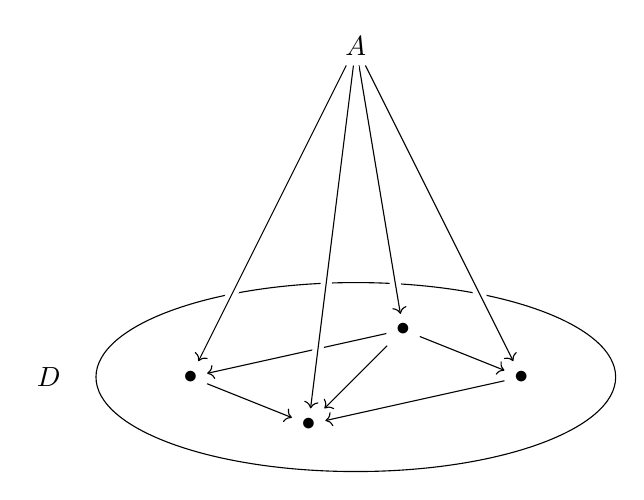
\begin{tikzpicture}[scale=3]
          \node (A) at (0,0.4) {$A$};
          \node (D1) at (0.2,-0.8) {$\bullet$};
          \node (D2) at (-0.7,-1) {$\bullet$};
          \node (D3) at (0.7,-1) {$\bullet$};
          \node (D4) at (-0.2,-1.2) {$\bullet$};
          \draw [->] (A) -- (D2);
          \draw [->] (A) -- (D3);
          \draw [->] (A) -- (D4);
          \draw [->] (D1) -- (D2);
          \draw [->] (D2) -- (D4);
          \draw [->] (D1) -- (D3);
          \draw [->] (D3) -- (D4);
          \draw [->] (D1) -- (D4);
          \draw [->] (A) -- (D1);
          \draw (0,-1) circle [x radius=1.1cm, y radius=0.4cm];
          \node at (-1.3, -1) {$D$};
          \begin{scope}[link/.style={white,double=black,line width=1.8pt,double distance=0.4pt, shorten > = 1.5mm}]
            \draw [link] (A) -- (D1);
            \draw [link] (A) -- (D2);
            \draw [link] (A) -- (D3);
            \draw [link] (A) -- (D4);
          \end{scope}
        \end{tikzpicture}
      \end{center}
      Given cones $(A, (\lambda_j)_{j \in \ob J})$ and $(B, (\mu_j)_{j \in \ob J})$, a morphism of cones between them is a morphism $A \overset{f}\to B$ such that
      \begin{equation*}
        \begin{tikzcd}[column sep=small]
          A \arrow[rr, "f"] \arrow[dr, "\lambda_j"'] && B \arrow[dl, "\mu_j"] \\
                                                    & D(j)
        \end{tikzcd}
      \end{equation*}
      commutes for all $j$.

      We write $\mathbf{Cone}(D)$ for the category of cones over $D$.
    \item \index{limit}\index{colimit}\hypertarget{def:limit} A \textbf{limit} for $D$ is a \hyperlink{def:terminal}{terminal object} of $\mathbf{Cone}(D)$, if this exists.
      Dually, we have the notion of \textbf{cone under a diagram}, and of \textbf{colimit} (\hyperlink{def:initial}{initial} cone under $D$).
  \end{enumerate}
\end{ndef}

Alternatively if $\mathscr{C}$ is \hyperlink{def:lsmall}{locally small} and $J$ is small, we have a \hyperlink{def:funct}{functor} $\mathscr{C}^{\hyperlink{def:duality}{\text{op}}} \to \mathbf{Set}$ sending $A$ to the set of \hyperlink{def:cone}{cones} with apex $A$.
A \hyperlink{def:limit}{limit} for $D$ is a \hyperlink{def:repr}{representation} of this functor.

If $\Delta A$ denotes the constant diagram of shape $J$ with all vertices $A$ and all edges $1_A$, then a \hyperlink{def:cone}{cone} over $D$ with \hyperlink{def:cone}{apex} $A$ is the same thing as a \hyperlink{def:nattrans}{natural transformation} $\Delta A \to D$.
$\Delta$ is a functor $\mathscr{C} \to [J, \mathscr{C}]$, and $\mathbf{Cone}(D)$ is the category $(\Delta \downarrow D)$ (a \hyperlink{def:comma}{comma category}, reversed).
So to say that every \hyperlink{def:diagram}{diagram of shape $J$} in $\mathscr{C}$ has a \hyperlink{def:limit}{limit} is equivalent to saying that $\Delta$ has a \hyperlink{def:adj}{right adjoint}.
\hypertarget{def:haslimits}(We say $\mathscr{C}$ \named{has limits} of shape $J$).
Dually, $\mathscr{C}$ \textbf{has colimits} of shape $J$ iff $\Delta: \mathscr{C} \to [J, \mathscr{C}]$ has a left adjoint.
\begin{nexample}\leavevmode
  \begin{enumerate}[label=(\alph*)]\label{eg:4.2}
    \item Suppose $J = \emptyset$. There's a unique \hyperlink{def:diagram}{diagram of shape $J$} in $\mathscr{C}$; a \hyperlink{def:cone}{cone} over it is just an object, and a morphism of cones is a morphism of $\mathscr{C}$.
      So a \hyperlink{def:limit}{limit} for this empty diagram is a \hyperlink{def:terminal}{terminal object} of $\mathscr{C}$.
      (Dually, a \hyperlink{def:limit}{colimit} for it is an initial object).
    \item\marginnote{\emph{Lecture 10}}[0cm]
      Let $J$ be the category
      \begin{equation*}
        \begin{tikzcd}
          \bullet & \bullet
        \end{tikzcd}
      \end{equation*}
      \index{span}\index{cospan}\hypertarget{def:span}A \hyperlink{def:diagram}{diagram of shape $J$} is a pair of objects $A,B$; a \hyperlink{def:cone}{cone} over it is a \textbf{span}
      \begin{equation*}
        \begin{tikzcd}[column sep=tiny]
          & \dlar C \drar  \\
          A && B
        \end{tikzcd}
      \end{equation*}
      and a \hyperlink{def:limit}{limit} for it is a \hyperlink{def:prod}{product}
      \begin{equation*}
        \begin{tikzcd}[column sep=tiny]
          & \arrow[dl, "\pi_1"'] A \times B \drar{\pi_2} \\
          A && B
        \end{tikzcd}
      \end{equation*}
      Dually, a colimit for it is a \hyperlink{def:coprod}{coproduct}
      \begin{equation*}
        \begin{tikzcd}[column sep=tiny]
        A \drar[']{\nu_1} && B \dlar{\nu_2} \\
          & A + B
        \end{tikzcd}
      \end{equation*}
    \item \hypertarget{def:lprod}More generally, if $J$ is a \hyperlink{def:small}{small} discrete category, a diagram of shape $J$ is a $J$-indexed family $\set{A_j | j \in J}$, and a limit for it is a product
      \begin{equation*}
        \Set{\prod_{j \in J} A_j \overset{\pi_j}\to A_j | j \in J}.
      \end{equation*}
      \hypertarget{def:lcoprod}Dually, a colimit for it is a coproduct
      \begin{equation*}
        \Set{A_j \overset{\nu_j}\to \sum_{j \in J} A_j | j \in J},
      \end{equation*}
      also written $\coprod_{j \in J} A_j$.
    \item Let $J$ be the category
      \begin{equation*}
        \begin{tikzcd}
          \bullet \rar[shift left] \rar[shift right] & \bullet
        \end{tikzcd}
      \end{equation*}
      A diagram of shape $J$ is a parallel pair
      \begin{equation*}
      \begin{tikzcd}
        A \rar[shift left]{f} \rar[shift right, ']{g} & B
      \end{tikzcd}
      \end{equation*} a cone over this is
      \begin{equation*}
        \begin{tikzcd}[column sep=tiny]
          & \arrow[dl, "h"'] C \drar{k} \\
          A && B
        \end{tikzcd}
      \end{equation*}
      satisfying $fh = k = gh$, or equivalently a morphism $C \overset{h}\to A$ satisfying $fh = gh$.
      A (co)limit for the diagram is a \hyperlink{def:equalizer}{(co)equalizer}.
    \item Let $J$ be the category
      \begin{equation*}
        \begin{tikzcd}
          & \bullet \dar \\
          \bullet \rar & \bullet
        \end{tikzcd}
      \end{equation*}
      A diagram of shape $J$ is a \hyperlink{def:span}{cospan}
      \begin{equation*}
        \begin{tikzcd}
          & A \dar{f} \\
          B \rar[']{g} & C
        \end{tikzcd}
      \end{equation*}
      a cone over it is
      \begin{equation*}
        \begin{tikzcd}
          D \rar{p} \dar{q} \drar{r} & A \\
          B & C
        \end{tikzcd}
      \end{equation*}
      satisfying $fp = r = gq$, or equivalently a span $(p,q)$ completing the diagram to a commutative square.
      \hypertarget{def:pullback}A limit for the diagram is called a \textbf{pullback} of $(f,g)$.
      In $\mathbf{Set}$, the \hyperlink{def:cone}{apex} of the pullback is the `fibre product'
      \begin{equation*}
        A \times_C B = \set{(x,y) \in A \times B | f(x) = g(y)}
      \end{equation*}
      \hypertarget{def:pushout}Dually, colimits of shape $J^{\text{op}}$ are called \textbf{pushouts}, given
      \begin{equation*}
        \begin{tikzcd}
          A \rar{f} \dar{g} & B \\
          C
        \end{tikzcd}
      \end{equation*}
      we `push $g$ along $f$' to get the right hand side of the colimit square.
      \item Let $J$ be the poset of natural numbers.
        A diagram of shape $J$ is a \textbf{direct system}
        \begin{equation*}
          \begin{tikzcd}
            A_0 \rar{f_0} & A_1 \rar{f_1} & A_2 \rar{f_2} & A_3 \rar{f_3} & \dots
          \end{tikzcd}
        \end{equation*}
        A colimit for this is called a \textbf{direct limit}: it consists of $A_\infty$ equipped with morphisms $A_n \overset{g_n} \to A_\infty$ satisfying $g_n = g_{n+1} f_n$ for all $n$, and universal among such.
        Dually, we have \textbf{inverse system} and \textbf{inverse limit}.
  \end{enumerate}
\end{nexample}
\begin{nthm}\label{thm:4.3}\leavevmode
  \begin{enumerate}[label=(\roman*)]
    \item Suppose $\mathscr{C}$ has \hyperlink{def:equalizer}{equalizers} and all finite (resp.\ \hyperlink{def:small}{small}) \hyperlink{def:lprod}{products}.
      Then $\mathscr{C}$ \hyperlink{def:haslimits}{has} all finite (resp.\ small) \hyperlink{def:limit}{limits}.
    \item Suppose $\mathscr{C}$ has \hyperlink{def:pullback}{pullbacks} and a \hyperlink{def:terminal}{terminal object}.
      Then $\mathscr{C}$ \hyperlink{def:haslimits}{has} all finite limits.
  \end{enumerate}
\end{nthm}
\begin{proof}\leavevmode
  \begin{enumerate}[label=(\roman*)]
    \item Suppose given $D: J \to \mathscr{C}$.
      Form the \hyperlink{def:lprod}{products}
      \begin{equation*}
        P = \prod_{j \in \ob J} D(j) \quad \text{and}\quad
        Q = \prod_{\alpha\in\mor J} D(\cod \alpha).
      \end{equation*}
    We have morphisms $\begin{tikzcd}P \rar[shift left]{f} \rar[shift right,']{g} & Q\end{tikzcd}$ defined by $\pi_\alpha f = \pi_{\cod \alpha}$, $\pi_\alpha g = D(\alpha) \pi_{\dom \alpha}$ for all $\alpha$.

    Let $E \overset{e}\to P$ be an \hyperlink{def:equalizer}{equalizer} of $(f,g)$.
    The composites $\lambda_j = \pi_j e: E \to D(j)$ form a \hyperlink{def:cone}{cone} over $D$:
    given $\alpha: j \to j'$ in $J$,
    \begin{equation*}
      D(\alpha) \lambda_j = D(\alpha) \pi_j e = \pi_\alpha g e = \pi_\alpha f e = \pi_{j'} e = \lambda_{j'}.
    \end{equation*}

    Given any cone $(A, \set{\mu_j | j \in \ob J})$ over $D$, there's a unique $\mu: A \to P$ with $\pi_j \mu = \mu_j$ for each $j$, and
    \begin{equation*}
      \pi_\alpha f \mu = \mu_{\cod \alpha} = D(\alpha) \mu_{\dom \alpha} = \pi_\alpha g \mu
    \end{equation*}
    for all $\alpha$, and hence $f\mu = g\mu$, so $\exists ! \nu: A \to E$ with $e \nu = \mu$.
    So $(E, \set{\lambda_j | j \in \ob J})$ is a \hyperlink{def:limit}{limit cone}.
  \item It's enough to construct finite products and equalizers.
    But if $1$ is the \hyperlink{def:terminal}{terminal object}, then a pullback for
    \begin{equation*}
      \begin{tikzcd}
        & A \dar \\
        B \rar & 1
      \end{tikzcd}
    \end{equation*}
    has the universal property of a product $A \times B$, and we can form $\prod_{i=1}^n A_i$ inductively as $A_1 \times (A_2 \times (A_3 \times \dotsm (A_{n-1} \times A_n) \dotsm)).$

    Now, to form the equalizer of $\begin{tikzcd}A \rar[shift left]{f} \rar[shift right,']{g} & B\end{tikzcd}$, consider the \hyperlink{def:span}{cospan}
    \begin{equation*}
      \begin{tikzcd}
        &A \dar{(1_A,f)} \\
        A \rar{(1_A, g)} & A \times B.
      \end{tikzcd}
    \end{equation*}
    A cone over this consists of
    \begin{equation*}
      \begin{tikzcd}
      P \rar{h} \dar{k} & A \\ A
      \end{tikzcd}
    \end{equation*}
    satisfying $(1_A, f) h = (1_A, g) k$ or equivalently, $1_A h = 1_A k$ and $fh = gk$, or equivalently a morphism $P \overset{h}\to A$ satisfying $fh = gh$.
    So a pullback for $(1_A,f)$ and $(1_A, g)$ is an equalizer of $(f,g)$. \qedhere
   \end{enumerate}
\end{proof}
\begin{defi}[Complete]\index{complete}\hypertarget{def:complete}
  We say a \hyperlink{def:cat}{category} $\mathscr{C}$ is \named{complete} if it has all \hyperlink{def:small}{small} \hyperlink{def:limit}{limits}.
  (Dually, \textbf{cocomplete} = all small colimits).
\end{defi}
Set is \hyperlink{def:complete}{complete} and cocomplete: \hyperlink{def:lprod}{products} are Cartesian products, \hyperlink{def:lcoprod}{coproducts} are disjoint unions.
Similarly, $\hyperlink{def:categ}{\mathbf{Gp}}, \mathbf{AbGp}, \hyperlink{def:categ}{\mathbf{Rng}, \mathbf{Mod}_R}, \dotsc$ are all complete and cocomplete.
$\mathbf{Top}$ is also complete and cocomplete.
\begin{ndef}\label{def:4.4}
  Let $F: \mathscr{C} \to \mathscr{D}$ be a \hyperlink{def:funct}{functor}.
  \begin{enumerate}[label=(\alph*)]
    \item \hypertarget{def:plim}We say $F$ \textbf{preserves limits}\index{limit!preserved}\index{preserves limits} of \hyperlink{def:diagram}{shape $J$} if, given $D: J \to \mathscr{C}$ and a \hyperlink{def:limit}{limit} \hyperlink{def:cone}{cone} $(L, \set{\lambda_j | j \in \ob J})$ in $\mathscr{C}$, $(FL, \set{F \lambda_j | j \in \ob J})$ is a limit for $FD$.
    \item \hypertarget{def:rlim}We say $F$ \textbf{reflects limits}\index{limit!reflected}\index{reflects limits} of shape $J$ if, given $D: J \to \mathscr{C}$ and a cone $(L, (\lambda_j)_j)$ such that $(FL, (F\lambda_j)_j)$ is a limit for $FD$, then $(L, (\lambda_j)_j)$ is a limit for $D$.
    \item \hypertarget{def:clim}We say $F$ \textbf{creates limits}\index{limit!created}\index{creates limits} of shape $J$ if, given $D: J \to \mathscr{C}$ and a limit $(M, (\mu_j)_j)$ for $FD$, there exists a cone $(L, (\lambda_j)_j)$ over $D$ whose image under $F$ is isomorphic to the limit cone, and any such that cone is a limit in $\mathscr{C}$.
  \end{enumerate}
\end{ndef}
\begin{nremark}\label{rem:4.5}\leavevmode\marginnote{\emph{Lecture 11}}[0cm]
  \begin{enumerate}[label=(\alph*)]
    \item If $\mathscr{C}$ has \hyperlink{def:limit}{limits of shape $J$}, $F: \mathscr{C} \to \mathscr{D}$ \hyperlink{def:plim}{preserves} them and $F$ reflects \hyperlink{def:iso}{isomorphisms}, then $F$ \hyperlink{def:rlim}{reflects} limits of shape $J$.
    \item $F$ reflects limits of shape $\mathbf{1} \iff F$ reflects isomorphisms.
      \item If $\mathscr{D}$ has limits of shape $J$ and $F: \mathscr{C} \to \mathscr{D}$ \hyperlink{def:clim}{creates them}, then $F$ both preserves and reflects them.
        \item In any of the statements of \cref{thm:4.3}, we may replace both instances of `$\mathscr{C}$ has' by either `$\mathscr{C}$ has and $F: \mathscr{C} \to \mathscr{D}$ preserves' or `$\mathscr{D}$ has and $F: \mathscr{C} \to \mathscr{D}$ creates'.
  \end{enumerate}
\end{nremark}
\begin{nexample}\label{eg:4.6}\leavevmode
  \begin{enumerate}[label=(\alph*)]
    \item $U: \mathbf{Gp} \to \mathbf{Set}$ (\hyperlink{def:forgFunc}{forgetful}) \hyperlink{def:clim}{creates} all \hyperlink{def:small}{small} limits:
      Given a family $\set{G_i | i \in I}$ of groups, there's a unique group structure on $\prod_{i \in I} UG_i$ making the projections $\pi_i$ into homomorphisms and this makes it into a product in $\mathbf{Gp}$.
      Similarly for \hyperlink{def:equalizer}{equalizers}.

      But $U$ doesn't \hyperlink{def:plim}{preserve} \hyperlink{def:lcoprod}{coproducts}: $U(G * H) \ncong UG \sqcup UH$.
    \item $U: \mathbf{Top} \to \mathbf{Set}$ (forgetful) \hyperlink{def:plim}{preserves} all small limits and colimits, but doesn't \hyperlink{def:rlim}{reflect} them: if $L$ is a \hyperlink{def:limit}{limit} for $D: J \to \mathbf{Top}$, and $L$ is not discrete, there's another \hyperlink{def:cone}{cone} with \hyperlink{def:cone}{apex} $L_d$ mapping to the limit in $\mathbf{Set}$.
    \item The inclusion functor $I: \mathbf{AbGp} \to \mathbf{Gp}$ reflects coproducts but doesn't preserve them.
      The direct sum $A \oplus B$ (coproduct in $\mathbf{AbGp}$) is not normally \hyperlink{def:iso}{isomorphic} to the free product $A * B$; $A*B$ is not abelian unless either $A$ or $B$ is $\{e\}$, but if $A \cong \{e\}$ then $A * B \cong A \oplus B \cong B$.
  \end{enumerate}
\end{nexample}
\begin{nlemma}\label{lem:4.7}
  If $\mathscr{D}$ has \hyperlink{def:limit}{limits of shape $J$}, then so does the \hyperlink{def:functcat}{functor category} $[\mathscr{C}, \mathscr{D}]$ for any $\mathscr{C}$, and the \hyperlink{def:forgFunc}{forgetful functor} $[\mathscr{C}, \mathscr{D}] \to \mathscr{D}^{\ob \mathscr{C}}$ \hyperlink{def:clim}{creates them}.
\end{nlemma}
\begin{proof}
  Suppose we are given a \hyperlink{def:diagram}{diagram of shape $J$} in $\hyperlink{def:functcat}{[\mathscr{C}, \mathscr{D}]}$; think of it as a \hyperlink{def:funct}{functor} $D: J \times \mathscr{C} \to \mathscr{D}$.
  For each $A \in \ob \mathscr{C}$, let $(LA, \set{\lambda_{j,A} | j \in \ob J})$ be a \hyperlink{def:limit}{limit} \hyperlink{def:cone}{cone} for the diagram $D(-, A): J \to \mathscr{D}$.
  Given $A \overset{f}\to B$ in $\mathscr{C}$, the composites
  \begin{equation*}
    A \overset{\lambda_{j,A}}\to D(j,A)\overset{D(j,f)}\to D(j,B)
  \end{equation*}
  form a cone over $D(-,B)$, since the squares
  \begin{equation*}
    \begin{tikzcd}[column sep=large, row sep=huge]
      {D(j,A)} \arrow[r, "{D(j,f)}"] \arrow[d, "{D(\alpha,A)}"] & {D(j,B)} \arrow[d, "{D(\alpha,B)}"] \\
      {D(j',A)} \arrow[r, "{D(j',f)}"] & {D(j',B)}
    \end{tikzcd}
  \end{equation*}
  commute.
  So there's a unique $Lf: LA \to LB$ making
  \begin{equation*}
    \begin{tikzcd}[column sep=large, row sep=huge]
    LA \rar{\lambda_{j,A}} \dar{Lf} & D(j,A) \dar{D(j,f)} \\
    LB \rar{\lambda_{j,B}} & D(j,B)
    \end{tikzcd}
  \end{equation*}
  commute for all $j$.

  Uniqueness implies functoriality: given $g: B \to C$, $L(gf)$ and $(Lg)(Lf)$ are factorizations of the same cone through the limit $LC$.
  And this is the unique functor structure on $(A \mapsto LA)$ making the $\lambda_{j, -}$ into \hyperlink{def:nattrans}{natural transformations}.

  The cone $(L, \{\lambda_{j, -} \mid j \in \ob J\})$ is a limit: suppose given another cone $(M, \{\mu_{j,-} \mid j \in \ob J\})$, then for each $A$, $(MA, \set{\mu_{j,A} | j \in \ob J})$ is a cone over $D(-,A)$, so induces a unique $\alpha_A: MA \to LA$.
  Naturality of $\alpha$ follows from uniqueness of factorisations through a limit.
  So $(M, (\mu_j))$ factors uniquely through $(L, (\lambda_j))$.
\end{proof}
\begin{nremark}\label{rem:4.8}
  In any \hyperlink{def:cat}{category}, a morphism $A \overset f\to B$ is \hyperlink{def:monic}{monic} iff
  \begin{equation*}
    \begin{tikzcd}
      A \rar{1_A} \dar{1_A} & A \dar{f}\\ A \rar{f} & B
    \end{tikzcd}
  \end{equation*}
    is a \hyperlink{def:pullback}{pullback}.
    Hence any \hyperlink{def:funct}{functor} which preserves pullbacks preserves monomorphisms.
    In particular, if $\mathscr{D}$ has pullbacks, then monomorphisms in $\hyperlink{def:functcat}{[\mathscr{C}, \mathscr{D}]}$ are just pointwise monomorphisms.
\end{nremark}
\begin{nthm}\label{thm:4.9}
  Suppose $G: \mathscr{D} \to \mathscr{C}$ has a \hyperlink{def:adj}{left adjoint} $F$.
  Then $G$ \hyperlink{def:plim}{preserves} all \hyperlink{def:limit}{limits} which exist in $\mathscr{D}$.
\end{nthm}
\begin{proof}[Proof 1]
  Suppose $\mathscr{C}$ and $\mathscr{D}$ both have \hyperlink{def:limit}{limits of shape $J$}.
  We have a commutative diagram
  \begin{equation*}
    \begin{tikzcd}
      \mathscr{C} \rar{F} \dar{\Delta} & \mathscr{D} \dar{\Delta} \\
      \left[J, \mathscr{C}\right] \rar{[J,F]} & \left[J, \mathscr{D}\right]
    \end{tikzcd}
  \end{equation*}
  and all the \hyperlink{def:funct}{functors} in it have \hyperlink{def:adj}{right adjoints} (in particular $[J,F] \dashv [J, G]$).
  So by \cref{cor:3.6}, the diagram of right adjoints
  \begin{equation*}
    \begin{tikzcd}
      \mathscr{D} \rar{G} & \mathscr{C} \\
      \left[J, \mathscr{D}\right] \rar{[J,G]} \uar{\lim_J} & \left[J, \mathscr{C}\right] \uar{\lim_J}
    \end{tikzcd}
  \end{equation*}
  commutes up to \hyperlink{def:iso}{isomorphism}, i.e.\ $G$ \hyperlink{def:plim}{preserves limits} of shape $J$.
\end{proof}
\begin{proof}[Proof 2]
  Suppose given $D: J \to \mathscr{D}$ and a \hyperlink{def:limit}{limit} \hyperlink{def:cone}{cone} $(L, \set{L \overset{\lambda_j}\to D(j) | j \in \ob J})$.
  Given a cone $(A, \set{A \overset{\alpha_j} \to GD(j) | j \in \ob J})$ over $GD$ the morphisms $FA \overset{\hat{\alpha_j}}\to D(j)$ form a cone over $D$, so they induce a unique $FA \overset{\hat{\beta}}\to L$ such that $\lambda_j \hat{\beta} = \hat{\alpha_j}$ for all $j$.
  Then $A \overset{\beta}\to GL$ is the unique morphism satisfying $(G\lambda_j) \beta = \alpha_j$ for all $j$.
  So $(GL, \set{G\lambda_j | j \in \ob J})$ is a limit cone in $\mathscr{C}$.
\end{proof}
\leavevmode\marginnote{\emph{Lecture 12}}[0cm]
\hypertarget{thm:paft}The \index{Adjoint Functor Theorem!Primeval}`Primeval' Adjoint Functor Theorem says that the converse of \cref{thm:4.9} is true: if $\mathscr{D}$ has and $G: \mathscr{D} \to \mathscr{C}$ \hyperlink{def:plim}{preserves} \emph{all} limits, then $G$ has a \hyperlink{def:adj}{left adjoint}.
\begin{nlemma}\label{lem:4.10}
  Suppose $\mathscr{D}$ \hyperlink{def:haslimits}{has} and $G: \mathscr{D} \to \mathscr{C}$ \hyperlink{def:plim}{preserves limits} of shape $J$.
  Then for any $A \in \ob \mathscr{C}$, the \hyperlink{def:comma}{arrow category} $(A \downarrow G)$ has \hyperlink{def:limit}{limits} of shape $J$, and the \hyperlink{def:forgFunc}{forgetful functor} $U: (A \downarrow G) \to \mathscr{D}$ \hyperlink{def:clim}{creates them}.
\end{nlemma}
\begin{proof}
  Suppose given $D : J \to (A \downarrow G)$, write $D(j)$ as $(U D(j), f_j)$.
  Let $(L, (\lambda_j: L \to U D(j))_{j \in \ob J})$ be a \hyperlink{def:limit}{limit} for $UD$;
  then $(GL, (G\lambda_j)_{j \in \ob J})$ is a limit for $GUD$.

  Since the edges of $UD$ are morphisms in $(A \downarrow G)$, the $f_j$ form a \hyperlink{def:cone}{cone} over $GUD$.
  So there's a unique $h: A \to GL$ such that $(G\lambda_j) h = f_j$ for all $j$,
  i.e.\ there's a unique $h$ such that the $\lambda_j$ are all morphisms $(L,h) \to (UD(j), f_j)$ in $(A \downarrow G)$.

  If $((C, k) (\mu_j)_{j \in \ob J})$ is any cone over $D$, then $(C, (\mu_j)_{j \in \ob J})$ is a cone over $UD$, so there's a unique $l: C \to L$ with $\lambda_j l = \mu_j$ for all $j$.
  We need to show $(Gl)k = h$:
  but $(G\lambda_j) (Gl) k = (G\mu_j) k = f_j = (G\lambda_j) h$
  for all $j$ so $(Gl)k = h$ by uniqueness of factorizations through limits.
\end{proof}
\begin{nlemma}\label{lem:4.11}
  A \hyperlink{def:cat}{category} $\mathscr{C}$ has an \hyperlink{def:initial}{initial object} iff $1_\mathscr{C}: \mathscr{C} \to \mathscr{C}$, regarded as a \hyperlink{def:diagram}{diagram} of shape $\mathscr{C}$ in $\mathscr{C}$, has a \hyperlink{def:limit}{limit}.
\end{nlemma}
\begin{proof}
  Suppose $\mathscr{C}$ has an \hyperlink{def:initial}{initial object} $I$.
  Then the unique morphisms
  $\set{I \to A \mid A \in \ob \mathscr{C}}$
  form a \hyperlink{def:cone}{cone} over $1_\mathscr{C}$; and given any cone $\Set{C \overset{\lambda_A}\to A | A \in \ob \mathscr{C}}$, then for any $A$ the triangle
  \begin{equation*}
    \begin{tikzcd}[sep=large]
      C \rar{\lambda_I} \drar[']{\lambda_A} & I \dar \\& A
    \end{tikzcd}
  \end{equation*}
  commutes, so $\lambda_I$ is the unique factorization of $\set{\lambda_A | A \in \ob \mathscr{C}}$ through the cone \begin{equation*}\set{I \to A \mid A \in \ob \mathscr{C}}.\end{equation*}

  Conversely, suppose $(I, \set{\lambda_A: I \to A| A \in \ob \mathscr{C}})$ is a \hyperlink{def:limit}{limit}.
  Then, for any $I \overset{f}\to A$, the diagram
  \begin{equation*}
    \begin{tikzcd}
      I \rar{\lambda_I} \drar[']{\lambda_A} & I \dar{f} \\ & A
    \end{tikzcd}
  \end{equation*}
  commutes.
  In particular, putting $f = \lambda_A$, we see that $\lambda_I$ is a factorization of the limit cone through itself, so $\lambda_I = 1_I$.
  Hence every $f: I \to A$ satisfies $f = \lambda_A$.
\end{proof}

The \hyperlink{thm:paft}{primeval Adjoint Functor Theorem} now follows immediately from \cref{lem:4.10}, \cref{lem:4.11} and \cref{thm:3.3}.
However, it only applies to \hyperlink{def:funct}{functors} between preorders (cf question 6 on example sheet 2).

\begin{nthm}[General Adjoint Functor Theorem]\label{thm:4.12gaft}
  Suppose that $\mathscr{D}$ is \hyperlink{def:lsmall}{locally small} and \hyperlink{def:complete}{complete}.
  \hypertarget{def:ssc}Then $G: \mathscr{D} \to \mathscr{C}$ has a \hyperlink{def:adj}{left adjoint} if and only if $G$ satisfies the \named{solution set condition}: the solution set condition says that $G$ preserves all small limits and, for each $A \in \ob \mathscr{C}$ there exists a set of morphisms $\set{A \overset{f_i}\to GB_i | i \in I}$ such that every $A \overset{h}\to GC$ factors as $A \overset{f_i}\to GB_i \overset{Gg}\to GC$ for some $i$ and some $g: B_i \to C$.
\end{nthm}
\begin{proof}
  $(\Rightarrow)$. If \hyperlink{def:adj}{$F \dashv G$}, $G$ \hyperlink{def:plim}{preserves limits} by \cref{thm:4.9}, and $\{A \overset{\eta_A}\to GFA\}$ is a singleton \hyperlink{def:ssc}{solution set}, by \cref{thm:3.3}.

  $(\Leftarrow)$. By \cref{lem:4.10}, $\hyperlink{def:comma}{(A \downarrow G)}$ is \hyperlink{def:complete}{complete}, and it inherits \hyperlink{def:lsmall}{local smallness} from $\mathscr{D}$.
  \hypertarget{def:winitial}So we need to show: if $\mathscr{A} \coloneqq (A \downarrow G)$ is complete and locally small, and has a weakly initial set of objects $\set{B_i | i \in I}$, then $\mathscr{A}$ has an initial object. (An object is \named{weakly initial} if it has a (not necessarily unique) morphism to any other object.)

  First form $P = \prod_{i \in I} B_i$, then $P$ is \hyperlink{def:winitial}{weakly initial}.
  Now form the limit of
  \begin{equation*}
    \begin{tikzcd}[column sep=huge]
    P \rar[shift left=0.5] \rar[shift left=2] \rar[shift left=3.5] \rar[shift right=3.5] \arrow[r, shift right=0.75, phantom, "\scriptscriptstyle\vdots"] & P
    \end{tikzcd} \tag{$*$}\label{eq:12star}
  \end{equation*}
  where edges are all the endomorphisms of $P$: denote the limit $I \overset{i}\to P$.
  $I$ is also \hyperlink{def:winitial}{weakly initial} in $\mathscr{A}$: suppose given $\begin{tikzcd}I \rar[shift left]{f} \rar[shift right,']{g} & C\end{tikzcd}$.
  Form the equalizer $E \overset{e}\to I$ of $(f,g)$, then there exists $P \overset{h}\to E$ since $P$ is weakly initial.
  $ieh:P \to P$, and $1_P$ are edges of the diagram \eqref{eq:12star} so $i = iehi$. But $i$ is monic, so $ehi = 1_I$, so $e$ is split epic, so $f = g$.
  Hence $I$ is initial.
\end{proof}
\begin{nexample}\label{eg:4.13}\leavevmode
  \begin{enumerate}[label=(\alph*)]
    \item Consider the \hyperlink{def:forgFunc}{forgetful functor} $U: \mathbf{Gp} \to \mathbf{Set}$.
      By \cref{eg:4.6}(a), $U$ creates all small limits, so $\mathbf{Gp}$ has them and $U$ preserves them.
      $\mathbf{Gp}$ is \hyperlink{def:lsmall}{locally small}, given a set $A$, any $f: A \to UG$ factors as $A \to UG' \to UG$, where $G'$ is the subgroup generated by $\set{f(x) | x \in A}$ and $\operatorname{card} G' \leq \max\{\aleph_0, \operatorname{card} A\}$.

      Let $B$ be a set of this cardinality; consider all subsets $B' \subseteq B$, all group structures on $B'$, and all mappings $A \to B'$.
      These give us a \hyperlink{def:ssc}{solution set} at $A$.
    \item Consider the category $\mathbf{CLat}$ of complete lattices (posets with all meets and joins).
      Again $U: \mathbf{CLat} \to \mathbf{Set}$ creates all small limits.
      But A.\ W.\ Hales (1964) showed that, for any cardinal $\kappa$, there exist complete lattices of $\operatorname{card} \geq\kappa$ generated by three elements, so the \hyperlink{def:ssc}{solution set condition} fails at $A = \{x,y,z\}$, and $U$ doesn't have a left adjoint.
  \end{enumerate}
\end{nexample}

\begin{ndef}[Subobject]\label{def:4.14}\hypertarget{def:subobj}
  By\marginnote{\emph{Lecture 13}}[0cm] a \named{subobject} of an object $A$ of $\mathscr{C}$, we mean a \hyperlink{def:monic}{monomorphism} $\begin{tikzcd}[cramped, sep=small]A' \rar[tail] & A\end{tikzcd}$.
  Dually, we have quotient objects.
  The subobjects of $A$ are preordered by $A'' \leq A'$ if there exists a factorization
  \begin{equation*}
    \begin{tikzcd}[column sep=small]
    A'' \drar[tail] \arrow[rr] && A' \arrow[ld, tail] \\
                            & A.
    \end{tikzcd}
  \end{equation*}

  \hypertarget{def:wp}We say $\mathscr{C}$ is \named{well-powered} if each $A \in \ob \mathscr{C}$ has a set of subobjects $\set{A_i \rightarrowtail  A | i \in I}$ such that every subobject of $A$ is isomorphic to some $A_i$ (e.g.\ in $\mathbf{Set}$ we can take the inclusions $\set{A' \hookrightarrow A | A' \in \mathcal{P}A}$).

  If $C^{op}$ is well-powered, we say $\mathscr{C}$ is \textbf{well-copowered} (not cowell-powered).
\end{ndef}
\begin{nlemma}\label{lem:4.15}
  Suppose given a \hyperlink{def:pullback}{pullback} square
  \begin{equation*}
    \begin{tikzcd}
      P \rar{h} \dar{k} & A \dar[tail]{f} \\
      B \rar{g} & C
    \end{tikzcd}
  \end{equation*}
  with $f$ \hyperlink{def:monic}{monic}. Then $k$ is monic.
\end{nlemma}
\begin{proof}
  Suppose $\begin{tikzcdi}D \rar[shift left]{x} \rar[shift right, ']{y} & P\end{tikzcdi}$ satisfy $kx = ky$.
  Then $fhx = gkx = gky = fhy$, but $f$ is \hyperlink{def:monic}{monic} so $hx = hy$.
  So $x$ and $y$ are factorizations of the same \hyperlink{def:cone}{cone} through the \hyperlink{def:limit}{limit} cone $(h,k)$.
\end{proof}
\begin{nthm}[Special adjoint functor theorem]\label{thm:4.16saft}
  Suppose $\mathscr{C}$ and $\mathscr{D}$ are both \hyperlink{def:lsmall}{locally small}, and that $\mathscr{D}$ is \hyperlink{def:complete}{complete} and \hyperlink{def:wp}{well-powered} and has a \hyperlink{def:separating}{coseparating} set.
  Then a \hyperlink{def:funct}{functor} $G:\mathscr{D}\to\mathscr{C}$ has a \hyperlink{def:adj}{left adjoint} iff it \hyperlink{def:plim}{preserves} all \hyperlink{def:limit}{small limits}.
\end{nthm}
\begin{proof}
  ($\Rightarrow$) by \cref{thm:4.9}.

  ($\Leftarrow$). For any $A \in \ob \mathscr{C}$, $(A \downarrow G)$ is \hyperlink{def:complete}{complete} by \cref{lem:4.10}, \hyperlink{def:lsmall}{locally small}, and \hyperlink{def:wp}{well-powered} since the \hyperlink{def:subobj}{subobjects} of $(B,f)$ in $(A \downarrow G)$ are just those \hyperlink{def:subobj}{subobjects} $B' \rightarrowtail B$ in $\mathscr{D}$ for which $f$ factors through $GB' \rightarrowtail GB$.

  Also, if $\set{S_i | i \in I}$ is a \hyperlink{def:separating}{coseparating} set for $\mathscr{D}$, then the set
  \begin{equation*}\set{(s_i, f) | i \in I, f \in \mathscr{C}(A, GS_i)}\end{equation*}
  is coseparating in $(A \downarrow G)$:
  given $\begin{tikzcdi}(B,f) \rar[shift left]{g}\rar[shift right, ']{h} & (B',f')\end{tikzcdi}$ in $(A \downarrow G)$ with $g \neq h$, there exists $k: B' \to S_i$ for some $i$ with $kg \neq kh$, and then $k$ is also a morphism $(B', f') \to (S_i, (Gk) f')$ in $(A\downarrow G)$.

  So we need to show that if $\mathscr{A}$ is complete, locally small and well powered, and has a coseparating set $\set{S_i | i \in I}$ then $\mathscr{A}$ has an initial object.
  Form the product $P = \prod_{i \in I} S_i$. Now consider the diagram
  \begin{center}
    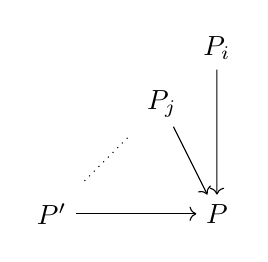
\begin{tikzpicture}[scale=0.7]
      \node (P1) at (3,3) {$P_i$};
      \node (P2) at (2,2) {$P_j$};
      \node (Pn) at (0,0) {$P'$};
      \node (P) at (3,0) {$P$};
      \draw [->] (P1) -- (P);
      \draw [->] (P2) -- (P);
      \draw [->] (Pn) -- (P);
      \draw [dotted, shorten < = 2mm, shorten > = 2mm] (P2) -- (Pn);
    \end{tikzpicture}
  \end{center}
  whose edges are a representative set of subobjects of $P$, and form its \hyperlink{def:limit}{limit}
  \begin{center}
    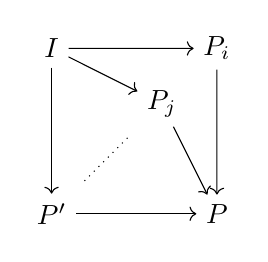
\begin{tikzpicture}[scale=0.7]
      \node (P1) at (3,3) {$P_i$};
      \node (P2) at (2,2) {$P_j$};
      \node (Pn) at (0,0) {$P'$};
      \node (P) at (3,0) {$P$};
      \draw [->] (P1) -- (P);
      \draw [->] (P2) -- (P);
      \draw [->] (Pn) -- (P);
      \node (I) at (0,3) {$I$};
      \draw [->] (I) -- (P1);
      \draw [->] (I) -- (P2);
      \draw [->] (I) -- (Pn);
      \draw [dotted, shorten < = 2mm, shorten > = 2mm] (P2) -- (Pn);
    \end{tikzpicture}
  \end{center}

  By the argument of \cref{lem:4.15}, the legs of this cone are all \hyperlink{def:monic}{monic}; in particular $I \rightarrowtail P$ is monic, and it's a \hyperlink{def:subobj}{least} subobject of $P$.
  Hence $I$ has no proper subobjects,
  so, given $\begin{tikzcdi}I \rar[shift left]{f} \rar[shift right,']{g} & A\end{tikzcdi}$, their \hyperlink{def:equalizer}{equalizer} is an \hyperlink{def:iso}{isomorphism} and hence $f = g$.

  Now let $A$ be any object of $\mathscr{A}$; form the \hyperlink{def:lprod}{product}
  \begin{equation*}
    Q = \prod_{\substack{i \in I \\ f \in \mathscr{A}(A,S_i)}} S_i.
  \end{equation*}
  There's an obvious $h: A \to Q$ defined by $\pi_{i,f} h = f$; and $h$ is monic, since the $S_i$ are a coseparating set.
  We also have a morphism $k : P \to Q$ defined by $\pi_{i,f} k = \pi_i$.

  Now form the \hyperlink{def:pullback}{pullback}
  \begin{equation*}
    \begin{tikzcd}
      B \rar \dar & A \dar[tail]{h} \\ P \rar{k} & Q
    \end{tikzcd};
  \end{equation*}
  by \cref{lem:4.15}, $B \to P$ is monic, so $B$ is a subobject of $P$.
  Hence there exists
  \begin{equation*}
    \begin{tikzcd}[column sep=small]
      I \arrow[rr] \drar[tail] && B \arrow[dl, tail] \\
                               & P
    \end{tikzcd}
  \end{equation*}
  and hence a morphism $I \to B \to A$.
\end{proof}
\begin{nexample}\label{eg:4.17}
  Consider the inclusion $\mathbf{KHaus} \overset{I}\to \mathbf{Top}$, where $\mathbf{KHaus}$ is the \hyperlink{def:fulls}{full subcategory} of compact Hausdorff spaces.
  $\mathbf{KHaus}$ \hyperlink{def:haslimits}{has} and $I$ \hyperlink{def:plim}{preserves} \hyperlink{def:small}{small} \hyperlink{def:lprod}{products} (by Tychonoff's Theorem) and \hyperlink{def:equalizer}{equalizers} (since equalizers of pairs $\begin{tikzcdi}X \rar[shift left]{f} \rar[shift right,']{g} & Y\end{tikzcdi}$ with $Y$ Hausdorff are closed subspaces).
  Both categories are \hyperlink{def:lsmall}{locally small} and $\mathbf{KHaus}$ is \hyperlink{def:wp}{well-powered} (subobjects of $X$ are all isomorphic to closed subspaces).
  The closed interval $[0,1]$ is a \hyperlink{def:separating}{coseparator} in $\mathbf{KHaus}$ by Urysohn's Lemma.
  So by \cref{thm:4.16saft}, $I$ has a \hyperlink{def:adj}{left adjoint} $\beta$.
\end{nexample}
\begin{nremark}\leavevmode
  \begin{enumerate}[label=(\alph*)]
    \item \v{C}ech's construction of $\beta$: given $X$ form $P = \prod_{f: X \to [0,1]} [0,1]$ and define $h: X \to P$ by $\pi_f h = f$.
      Define $\beta X$ to be the closure of the image of $h$.

      \v{C}ech's proof that this works is essentially the same as \cref{thm:4.16saft}.
    \item We could have used \nameref{thm:4.12gaft} to construct $\beta$: we get a solution set at $X$ by considering all continuous $X \overset{f}\to Y$ with $Y$ compact Hausdorff, and $\operatorname{im} f$ dense in $Y$ and such $Y$ have cardinality $\leq 2^{2^{\operatorname{card} X}}$.
  \end{enumerate}
\end{nremark}
\clearpage
\section{Monads}
Suppose given
\marginnote{\emph{Lecture 14}}[0cm]
\begin{equation*}
  \begin{tikzcd}
    \mathscr{C} \rar[shift left]{F} & \mathscr{D} \lar[shift left]{G}
  \end{tikzcd}
\end{equation*}
with $\hyperlink{def:adj}{(F \dashv G)}$.
How much of this structure can we describe without mentioning $\mathscr{D}$?

We have the \hyperlink{def:funct}{functor} $T= GF: \mathscr{C} \to \mathscr{C}$, and the \hyperlink{def:unit}{unit} $\eta: 1_\mathscr{C} \to T = GF$ and the \hyperlink{def:nattrans}{natural transformation}
\begin{equation*}
  \mu = G\epsilon_F: TT = GFGF \to GF = T.
\end{equation*}
These satisfy the commutative diagrams

\begin{equation*}
  \begin{tikzcd}[sep=large]
    T \rar{T\eta} \arrow[dr, "1_T"'{name=mid}]
    & TT \arrow[d, "\mu"{name=here}] & T \lar[']{\eta_T} \arrow[dl, "1_T"]\\
    & T \arrow[from=1-1, to=here, "\hypertarget{eq:monad1}\scriptstyle(1)" description, pos=0.67, phantom]\arrow[from=1-3, to=here, "\hypertarget{eq:monad2}\scriptstyle(2)" description, pos=0.67, phantom]
  \end{tikzcd}
\end{equation*}
by \hyperlink{def:triId}{triangular identities} and
\begin{equation*}
  \begin{tikzcd}[row sep=large]
  TTT \rar{T\mu} \dar{\mu_T} \arrow[dr, phantom, "\hypertarget{eq:monad3}\scriptstyle(3)" description]& TT \dar{\mu} \\
    TT \rar{\mu} & T
  \end{tikzcd}
\end{equation*}
by naturality of $\epsilon$.

\begin{ndef}[Monad]\hypertarget{def:monad}
  A \named{monad} $\mathbb{T} = (T, \eta, \mu)$ on a \hyperlink{def:cat}{category} $\mathscr{C}$ consists of a \hyperlink{def:funct}{functor} $T: \mathscr{C} \to \mathscr{C}$ and \hyperlink{def:nattrans}{natural transformation} $\eta: 1_\mathscr{C} \to T$, $\mu: TT \to T$ satisfying equations \hyperlink{eq:monad1}{(1)}-\hyperlink{eq:monad3}{(3)}.
  $\eta$ and $\mu$ are called the \textbf{unit} and \textbf{multiplication} of $\mathbb{T}$.
\end{ndef}
\begin{nexample}\leavevmode
  \begin{enumerate}[label=(\alph*)]\label{eg:5.2}
    \item Any \hyperlink{def:adj}{adjunction} $(F \dashv G)$ induces both a \hyperlink{def:monad}{monad} $(GF, \eta, G\epsilon_F)$ on $\mathscr{C}$ and a \hyperlink{def:duality}{co}monad $(FG, \epsilon, F\eta_G)$ on $\mathscr{D}$.
    \item Let $M$ be a \hyperlink{def:monoid}{monoid}. The functor $(M \times -): \mathbf{Set} \to \mathbf{Set}$ has a monad structure with \hyperlink{def:monad}{unit} given by $\eta_A(a) = (1_M, a)$ and \hyperlink{def:monad}{multiplication} $\mu_A(m, m', a) = (mm', a)$.
      The monad identities follow from the monoid ones.
    \item Let $\mathscr{C}$ be any \hyperlink{def:cat}{category} with finite \hyperlink{def:lprod}{products}, $A \in \ob \mathscr{C}$.
      The \hyperlink{def:funct}{functor} $(A \times -): \mathscr{C} \to \mathscr{C}$ has a comonad structure with counit $\epsilon_B : A \times B \to B$ given by $\pi_2$ and comultiplication $\delta_B: A \times B \to A\times A \times B$ given by $(\pi_1, \pi_1, \pi_2)$.
  \end{enumerate}
\end{nexample}
Does every \hyperlink{def:monad}{monad} arise from an \hyperlink{def:adj}{adjunction}?

In \cref{eg:5.2}(b) we have the \hyperlink{def:cat}{category} \hyperlink{def:functcat}{$[M, \mathbf{Set}]$}.
Its \hyperlink{def:forgFunc}{forgetful functor} to $\mathbf{Set}$ has a left \hyperlink{def:adj}{adjoint}, sending $A$ to $M \times A$ with $M$ acting by multiplication on the left factor.
This adjunction gives rise to the \hyperlink{def:monad}{monad} of \cref{eg:5.2}(b).

\begin{ndef}[Eilenberg-Moore category]\label{def:5.3}
  \hypertarget{def:em}Let $\mathbb{T}$ be a \hyperlink{def:monad}{monad} on $\mathscr{C}$.
  A $\mathbb{T}$-\textbf{algebra}\index{Talgebra@$\mathbb{T}$-algebra} is a pair $(A, \alpha)$ with $A \in \ob \mathscr{C}$ and $TA \overset{\alpha}\to A$ satisfying the commutative diagrams
  \begin{equation*}
    \begin{tikzcd}[sep=large]
      A \rar{\eta_A} \drar[']{1_A} & TA \arrow[d, "\alpha"{name=here}] \\ & A
      \arrow[from=1-1, to=here, phantom, "\scriptstyle\hypertarget{eq:em4}(4)" description, pos=0.67]
    \end{tikzcd}
  \end{equation*}
  \begin{equation*}
    \begin{tikzcd}[sep=large]
      TTA \rar{T\alpha} \dar{\mu_A} \arrow[dr, phantom, "\hypertarget{eq:em5}\scriptstyle(5)" description] & TA \dar{\alpha} \\ TA \rar{\alpha} & A.
    \end{tikzcd}
  \end{equation*}
  A \textbf{homomorphism}\index{algebra!homomorphism} $f: (A, \alpha) \to (B, \beta)$ is a morphism $A \overset{f}\to B$ such that
  \begin{equation*}
    \begin{tikzcd}[sep=large]
      TA \rar{Tf} \dar{\alpha} \arrow[dr, phantom, "\hypertarget{eq:em6}\scriptstyle(6)" description] & TB \dar{\beta} \\ A \rar{f} & B
    \end{tikzcd}
  \end{equation*}
  commutes.
  The category of $\mathbb{T}$-algebras is denoted $\mathscr{C}^\mathbb{T}$, and called the \named{Eilenberg-Moore category}.
\end{ndef}
\begin{nlemma}\label{lem:5.4}\hypertarget{def:fsupt}
  The \hyperlink{def:forgFunc}{forgetful functor} $G^\mathbb{T}: \hyperlink{def:em}{\mathscr{C}^\mathbb{T}} \to \mathscr{C}$ has a \hyperlink{def:adj}{left adjoint} $F^\mathbb{T}$ and the adjunction induces $\mathbb{T}$.
\end{nlemma}
\begin{proof}
  We define $F^\mathbb{T} A = (TA, \mu_A)$ (an \hyperlink{def:em}{algebra} by \hyperlink{eq:monad2}{(2)} and \hyperlink{eq:monad3}{(3)}) and $F^\mathbb{T}(A \overset{f}\to B) = Tf$ (a \hyperlink{def:em}{homomorphism} by \hyperlink{def:nattrans}{naturality} of $\mu$).

  Clearly $G^\mathbb{T} F^\mathbb{T} = T$, the \hyperlink{def:unit}{unit} of the \hyperlink{def:adj}{adjunction} is $\eta$.
  We define the \hyperlink{def:counit}{counit}
  \begin{equation*}\epsilon_{(A,a)} = \alpha: (TA, \mu_A) \to (A, \alpha)\end{equation*}
  (a homomorphism by \hyperlink{eq:em5}{(5)})
  $\epsilon$ is natural by \hyperlink{eq:em6}{(6)}; for the triangular identities, $\epsilon_{FA} (F \eta_A) = 1_{FA}$ is \hyperlink{eq:monad1}{(1)}, $G \epsilon_{(A,\epsilon)} \eta_A = 1_A$ is \hyperlink{eq:em4}{(4)}.

  The \hyperlink{def:monad}{monad} induced by $(F^\mathbb{T} \dashv G^\mathbb{T})$ has \hyperlink{def:funct}{functor} $T$ and unit $\eta$, and $G^\mathbb{T} \epsilon_{F^\mathbb{T} A} = \mu_A$ by definition of $F^\mathbb{T} A$.
\end{proof}

Kleisli took a `minimalist' approach: if
\begin{equation*}
  \begin{tikzcd}[column sep=large]
    \mathscr{C} \rar[shift left]{F} & \mathscr{D} \lar[shift left]{G}
  \end{tikzcd}
\end{equation*}
induces $\mathbb{T}$, then so does
\begin{equation*}
  \begin{tikzcd}[column sep=large]
    \mathscr{C} \rar[shift left]{F} & \mathscr{D}' \lar[shift left]{G|_{\mathscr{D}'}}
  \end{tikzcd}
\end{equation*}
where $\mathscr{D}'$ is the \hyperlink{def:fulls}{full subcategory} of $\mathscr{D}$ on objects $FA$.

So in trying to construct $\mathscr{D}$, we may assume $F$ is surjective (or indeed bijective) on objects.
But then morphisms $FA \to FB$ correspond bijectively to morphisms $A \to GFB = TB$ in $\mathscr{C}$.

\begin{ndef}[Kleisli category]\label{def:5.5}
  Given \hypertarget{def:kleisli}a \hyperlink{def:monad}{monad} $\mathbb{T}$ on $\mathscr{C}$, the \named{Kleisli category} $\mathscr{C}_\mathbb{T}$ has $\ob \mathscr{C}_{\mathbb{T}} = \ob \mathscr{C}$, and morphisms $A \green{\to} B$ are morphisms $A \to TB$ in $\mathscr{C}$.
  The composite $A \green{\overset{f}\to} B \green{\overset{g}\to} C$ is
  \begin{equation*}
    \begin{tikzcd}
      A \rar{f} & TB \rar{Tg} & TTC \rar{\mu_C} & TC
    \end{tikzcd}
  \end{equation*}
  and the identity $A \green{\to} A$ is $A \overset{\eta_A}\to TA$.

  To verify associativity, suppose given $A \green{\overset{f}\to} B \green{\overset{g}\to} C \green{\overset{h}\to} D$.
  Then
  \begin{equation*}
    \begin{tikzcd}[row sep=large]
    A \rar{f} & TB \rar{Tg} & TTC \rar{TTh} \dar{\mu_C} & TTTD \dar{\mu_{TD}} \rar{T \mu_D} \arrow[dr, "\scriptstyle\hyperlink{eq:monad3}{(3)}" description, phantom] & TTD \dar{\mu_D} \\
                && TC \rar{Th} & TTD \rar{\mu_D} & TD
    \end{tikzcd}
  \end{equation*}
  commutes by naturality: the upper way round is $\green{(hg)f}$ and the lower is $\green{h(gf)}$.

  The unit laws for the \hyperlink{def:cat}{category} similarly follow from
  \begin{equation*}
    \begin{tikzcd}[row sep=large]
    A \rar{f} & TB \rar{T\eta_B} \drar[']{1_{TB}} & TTB \arrow[d, "\mu_B"{name=here}]  \\
              && TB \arrow[from=1-2, to=here, "\scriptstyle\hyperlink{eq:monad1}{(1)}" description, phantom, pos=0.67]
    \end{tikzcd}
  \end{equation*}
  and
  \begin{equation*}
    \begin{tikzcd}[row sep=large]
    A \rar{f} \dar{\eta_A} & TB \drar{1_{TB}} \dar[']{\eta_{TB}} \\
    TA \rar[']{Tf} & TTB \arrow[r,"\mu_B"'{name=here}] & TB.\arrow[from=1-2, to=here, "\scriptstyle\hyperlink{eq:monad2}{(2)}" description, phantom, pos=0.67]
    \end{tikzcd}
  \end{equation*}
\end{ndef}
\begin{nlemma}\label{lem:5.6}\hypertarget{def:fsubt}
  There \marginnote{\emph{Lecture 15}}exists an \hyperlink{def:adj}{adjunction}
  \begin{equation*}
    \begin{tikzcd}
      \mathscr{C} \rar[shift left]{F_\mathbb{T}} & \hyperlink{def:kleisli}{\mathscr{C}_\mathbb{T}} \lar[shift left]{G_\mathbb{T}}
    \end{tikzcd}
  \end{equation*}
  inducing the \hyperlink{def:monad}{monad} $\mathbb{T}$.
\end{nlemma}
\begin{proof}
  We define $F_\mathbb{T} A = A$,
  \begin{equation*}F_\mathbb{T}(A \overset{f}\to B) = A \overset{f}\to B \overset{\eta_B}\to TB.\end{equation*}
  $F_\mathbb{T}$ preserves identities by definition; for composites, consider $A \overset{f}\to B \overset{g}\to C$.
  We get
  \begin{equation*}
    \begin{tikzcd}[sep=large]
      A \rar{f} & B \dar{g} \rar{\eta_B} & TB \dar{Tg} \\
                & C \rar{\eta_C} & TC \rar{T\eta_c} \drar[']{1_{TC}} & TTC \arrow[d, "\mu_C"{name=me}] \\
                &&& TC. \arrow[from=2-3, to=me, "\scriptstyle\hyperlink{eq:monad1}{(1)}" description, phantom, pos=0.67]
    \end{tikzcd}
  \end{equation*}
  We define $G_\mathbb{T}A = TA$,
  \begin{equation*}
    G_\mathbb{T}(A \green{\overset{f}\to} B) = TA \overset{Tf}\to TTB \overset{\mu_B}\to TB.
  \end{equation*}
  $G_\mathbb{T}$ preserves identities by \hyperlink{eq:monad1}{(1)}; for composites, consider $A \green{\overset{f}\to} B \green{\overset{g}\to} C$.
  We get
  \begin{equation*}
    \begin{tikzcd}[row sep=large]
    TA \rar{Tf} & TTB \rar{TTg} \dar{\mu_B} & TTTC \arrow[dr, phantom, "\scriptstyle\hyperlink{eq:monad3}{(3)}" description]\rar{T\mu_C} \dar{\mu_{TC}} & TTC \dar{\mu_C} \\
                  & TB \rar{Tg} & TTC \rar{\mu_C} & TC
    \end{tikzcd}
  \end{equation*}
  We have
  \begin{gather*}G_\mathbb{T} F_\mathbb{T} A = TA \\ G_\mathbb{T} F_\mathbb{T} f = \mu_B (T\eta_B) Tf = Tf\end{gather*}
  so we take $\eta: 1_\mathbb{C} \to T$ as the \hyperlink{def:unit}{unit} of $\hyperlink{def:adj}{(F_\mathbb{T} \dashv G_\mathbb{T})}$.
  The counit $TA \green{\overset{\epsilon_A}\to} A$ is $1_{TA}$. To verify \hyperlink{def:nattrans}{naturality}, consider the square
  \begin{equation*}
    \begin{tikzcd}[sep=large]
      TA \rar[red]{F_\mathbb{T}G_\mathbb{T}f} \dar[red]{\epsilon_A} & TB \dar[red]{\epsilon_B} \\
      A \rar[red]{f} & B
    \end{tikzcd}
  \end{equation*}
  This expands to
  \begin{equation*}
    \begin{tikzcd}[row sep=large]
    TA \rar{Tf} & TTB \rar{\mu_B} & TB \rar{\eta_{TB}} \drar[']{1_{TB}} &TTB \arrow[d,"\mu_B"{name=me}] \\
                &               &                               &TB \arrow[from=1-3, to=me, "\scriptstyle\hyperlink{eq:monad2}{(2)}" description, phantom, pos=0.67]
    \end{tikzcd}
  \end{equation*}
  so $\epsilon$ is natural.
  \begin{equation*}
    G_\mathbb{T}(TA \green{\overset{\epsilon_A}\to} A) = \mu_A, \text{ so } G_\mathbb{T}(\green{\epsilon_A}) \eta_{G_\mathbb{T}A} = \mu_A \cdot \eta_{TA} = 1_{TA}
  \end{equation*}
  and $\green{(\epsilon_{F_\mathbb{T}A})(F_\mathbb{T}\eta_A)}$ is
  \begin{equation*}
    \begin{tikzcd}[row sep=large]
    A \rar{\eta_A} & TA \rar{\eta_{TA}} \drar[']{1_{TA}} & TTA \arrow[d, "\mu_A"{name=me}] \\ &&TA \arrow[from=1-2,to=me, phantom, "\scriptstyle\hyperlink{eq:monad1}{(1)}" description]
  \end{tikzcd}
  \end{equation*}
  which is $\green{1_{F_\mathbb{T}A}}$.
  Also $G_\mathbb{T}(\green{\epsilon_{F_\mathbb{T}A}}) = \mu_A$, so $(F_\mathbb{T} \dashv G_\mathbb{T})$ induces $\mathbb{T}$.
\end{proof}
\begin{nthm}\label{thm:5.7}
  Given a \hyperlink{def:monad}{monad} $\mathbb{T}$ on $\mathscr{C}$, let $\mathbf{Adj}(\mathbb{T})$ be the category whose objects are the \hyperlink{def:adj}{adjunctions}
  $\left(\begin{tikzcdi}\mathscr{C} \rar[shift left]{F} & \mathscr{D} \lar[shift left]{G}\end{tikzcdi}\right)$
  inducing $\mathbb{T}$, and whose morphisms
  \begin{equation*}\left(\begin{tikzcdi}\mathscr{C} \rar[shift left]{F} & \mathscr{D} \lar[shift left]{G}\end{tikzcdi}\right)\to \left(\begin{tikzcdi}\mathscr{C} \rar[shift left]{F'} & \mathscr{D}' \lar[shift left]{G'}\end{tikzcdi}\right)\end{equation*}
  are functors $H: \mathscr{D} \to \mathscr{D}'$ satisfying $HF = F'$ and $G'H = G$.
  Then the \hyperlink{def:kleisli}{Kleisli} \hyperlink{def:adj}{adjunction} is an \hyperlink{def:initial}{initial} object of $\mathbf{Adj}(\mathbb{T})$, and the \hyperlink{def:em}{Eilenberg-Moore} adjunction is \hyperlink{def:terminal}{terminal}.
\end{nthm}
\begin{proof}
  \hypertarget{def:emcomp}Let $\left(\begin{tikzcdi}\mathscr{C} \rar[shift left]{F} & \mathscr{D} \lar[shift left]{G}\end{tikzcdi}\right)$ be an object of $\mathbf{Adj}(\mathbb{T})$.
  We define $K: \mathscr{D} \to \hyperlink{def:em}{\mathscr{C}^\mathbb{T}}$ (the \textbf{Eilenberg-Moore comparison functor}) by $KB = (GB, G\epsilon_B)$ where $\epsilon$ is the \hyperlink{def:counit}{counit} of $(F \dashv G)$; note this is an \hyperlink{def:em}{algebra} by one of the \hyperlink{def:triId}{triangular identities} for $(F \dashv G)$ and \hyperlink{def:nattrans}{naturality} of $\epsilon$ and $K(B \overset{g}\to B') = Gg$ (a homomorphism by naturality of $\epsilon$).
  Clearly $\hyperlink{def:fsupt}{G^\mathbb{T}}K = G$ and
  \begin{gather*}KFA = (GFA, G\epsilon_{FA}) = (TA, \mu_A) = \hyperlink{def:fsupt}{F^\mathbb{T}}A,\\
  KF(A\overset{f}\to A') = Tf = F^\mathbb{T} f.\end{gather*}
  So $K$ is a morphism of $\mathbf{Adj}(\mathbb{T})$.

  Suppose $K': \mathscr{D} \to \mathscr{C}^\mathbb{T}$ is another such; then since $G^\mathbb{T} K' = G$, we know $K' B = (GB, \beta_B)$ where $\beta$ is a natural transformation $GFG \to G$.
  Also, since $K'F = F^\mathbb{T}$, we have $\beta_{FA} = \mu_A = G\epsilon_{FA}$.

  Now, given any $B \in \ob \mathscr{D}$, consider the diagram
  \begin{equation*}
    \begin{tikzcd}[column sep=huge, row sep=scriptsize]
    GFGFGB \arrow[dd,shift right=2,',"G\epsilon_{FGB}"] \arrow[dd,shift left=2,"\beta_{FGB}"] \rar{GFG\epsilon_B} & GFGB \arrow[dd,shift right=2,',"G\epsilon_B"] \arrow[dd,shift left=2,"\beta_B"] \\ =\\
    GFGB \rar{G\epsilon_B} & GB
  \end{tikzcd}
  \end{equation*}
  Both squares commute so $G\epsilon_B$ and $\beta_B$ have the same composite with $GFG\epsilon_B$.
  But this is \hyperlink{def:split}{split} \hyperlink{def:epic}{epic}, with splitting $GF\eta_{GB}$, so $\beta = G\epsilon$. Hence $K' = K$.

  \hypertarget{def:klcomp}We now define the \textbf{Kleisli comparison functor} $L: \hyperlink{def:kleisli}{\mathscr{C}_\mathbb{T}} \to \mathscr{D}$ by $LA = FA$,
  \begin{equation*}
  L(A \green{\overset{f}\to} B) =
  \begin{tikzcd}
    FA \rar{Ff} & FGFB \rar{\epsilon_{FB}} & FB.
  \end{tikzcd}
  \end{equation*}
  $L$ preserves identities by one of the \hyperlink{def:triId}{triangular identities} for $(F \dashv G)$; given $A \green{\overset{f}\to} B \green{\overset{g}\to} C$, we have
  \begin{equation*}
    \begin{tikzcd}[column sep=large, row sep=large]
    FA \rar{Ff} & FGFB \rar{FGFg} \dar{\epsilon_{FB}}& FGFGFC \dar{\epsilon_{FGFC}}\rar{FG\epsilon_{FC}}& FGFC \dar{\epsilon_{FC}} \\
                & FB \rar{Fg}& FGFC \rar{\epsilon_{FC}} & FC
  \end{tikzcd}
  \end{equation*}
  $GLA = TA = \hyperlink{def:fsubt}{G_\mathbb{T}}A$, \begin{equation*}GL(A \green{\overset{f}\to} B) = (G \epsilon_{FB}) (GFf) = \mu_B(Tf).\end{equation*}
  $L\hyperlink{def:fsubt}{F_\mathbb{T}}A = FA$, \begin{equation*}LF_\mathbb{T}(A \overset{f}\to B) = (\epsilon_{FB})(F\eta_B) (Ff) = Ff = G_{\mathbb{T}} f.\end{equation*}
  Note that $L$ is full and faithful; its effect on morphisms (with given domain and codomain) is that of transposition across $(F \dashv G)$.
  Suppose $L': \mathscr{C}_\mathbb{T} \to \mathscr{D}$ is a morphism of $\mathbf{Adj}(\mathbb{T})$.
  We must have $L'A = FA$, and $L'$ maps the counit $TA \green{\to} A$ to the counit $FGFA \overset{\epsilon_{FA}} \to FA$.
  For any $A \green{\overset{f}\to} B$, we have $\green{f}=\green{1_{TA} (F_\mathbb{T} f)}$ so $L'(\green{f}) = \epsilon_{FA} \cdot (Ff) = L\green{f}$.
\end{proof}
If \marginnote{\emph{Lecture 16}}$\mathscr{C}$ has \hyperlink{def:lcoprod}{coproducts}, then so does $\hyperlink{def:kleisli}{\mathscr{C}_\mathbb{T}}$, since $\hyperlink{def:fsubt}{F_\mathbb{T}}$ preserves them.
But in general, it has few other \hyperlink{def:limit}{limits} or colimits. In contrast, we have
\begin{nthm}\label{thm:5.8}\leavevmode
  \begin{enumerate}[label=(\roman*)]
    \item The \hyperlink{def:forgFunc}{forgetful functor} $G: \hyperlink{def:em}{\mathscr{C}^\mathbb{T}} \to \mathscr{C}$ \hyperlink{def:clim}{creates all limits} which exist in $\mathscr{C}$.
    \item If $\mathscr{C}$ \hyperlink{def:haslimits}{has colimits} of \hyperlink{def:limit}{shape $J$}, then $G: \mathscr{C}^\mathbb{T} \to \mathscr{C}$ creates them $\iff T$ \hyperlink{def:plim}{preserves them}.
  \end{enumerate}
\end{nthm}

\begin{proof}\leavevmode
  \begin{enumerate}[label=(\roman*)]
    \item Suppose given $D: J \to \mathscr{C}^\mathbb{T}$; write $D(j) = (GD(j), \delta_j)$ and suppose
      \begin{equation*}(L, \set{\mu_j: L \to GD(j) | j \in \ob J})\end{equation*}
      is a \hyperlink{def:limit}{limit cone} for $GD$.
      Then the composites
      \begin{equation*}
        \begin{tikzcd}
          TL \rar{T\mu_j} & TGD(j) \rar{\delta_j} & GD(j)
        \end{tikzcd}
      \end{equation*}
      form a cone over $GD$, since the edges of $GD$ are \hyperlink{def:em}{homomorphisms}, so they induce a unique $\lambda: TL \to L$ such that $\mu_j \lambda = \delta_j(T\mu)$ for all $j$.
      The fact that $\lambda$ is a \hyperlink{def:em}{$\mathbb{T}$-algebra} structure on $L$ follows from the fact that the $\delta_j$ are algebra structures and uniqueness of factorisations through limits.

      So $((L,\lambda), \set{\mu_j | j \in \ob J})$ is the unique lifting of the limit cone over $GD$ to a cone over $D$; and it's a limit, since given a cone over $D$ with apex $(A, \alpha)$, we get a unique factorisation $A \overset{f}\to L$ in $\mathscr{C}$ and $F$ is an algebra homomorphism by uniqueness of factorisations through $L$.

    \item $(\Rightarrow)$ $F: \mathscr{C} \to \mathscr{C}^\mathbb{T}$ \hyperlink{def:plim}{preserves colimits} since it's a \hyperlink{def:adj}{left adjoint}, so $T = GF$ preserves colimits of shape $J$.

      $(\Leftarrow)$ Suppose given $D: J \to \mathscr{C}^\mathbb{T}$ as in (i), and a colimit cone
      \begin{equation*}
        \set{GD(j) \overset{\mu_j}\to L | j \in \ob J}
      \end{equation*}
      in $\mathscr{C}$.
      Then
      \begin{equation*}
        \set{TGD(j) \xrightarrow{T\mu_j} TL | j \in \ob J}
      \end{equation*}
      is also a colimit cone, so the composites
      \begin{equation*}
        \begin{tikzcd}
          TGD(j) \rar{\delta_j} & GD(j) \rar{\mu_j}& L
        \end{tikzcd}
      \end{equation*}
      induce a unique $\lambda: TL \to L$.
      The rest of the argument is like (i). \qedhere
  \end{enumerate}
\end{proof}
\begin{ndef}[Monadic adjunction]\hypertarget{def:monadic}
  Given an \hyperlink{def:adj}{adjunction} $\left(\begin{tikzcdi}\mathscr{C} \rar[shift left]{F} & \mathscr{D} \lar[shift left]{G}\end{tikzcdi}\right)$, with $(F \dashv G)$ we say the adjunction (or the functor $G$) is \textbf{monadic} if the \hyperlink{def:emcomp}{comparison functor} $K : \mathscr{D} \to \mathscr{C}^\mathbb{T}$ is part of an \hyperlink{def:equicat}{equivalence} of \hyperlink{def:cat}{categories}.
\end{ndef}
(Note that, since the \hyperlink{def:klcomp}{Kleisli comparison} $\mathscr{C}_\mathbb{T} \to \mathscr{D}$ is \hyperlink{def:full}{full} and \hyperlink{def:full}{faithful}, it's part of an \hyperlink{def:equicat}{equivalence} if and only if it (equivalently, $F$) is \hyperlink{def:full}{essentially surjective} on objects.)
\begin{remark}
  Given any \hyperlink{def:adj}{adjunction} $(F \dashv G)$, for each object $B$ of $\mathscr{D}$ we have a diagram
  \begin{equation*}
    \begin{tikzcd}[column sep=large]
      FGFGB \rar[shift left]{FG\epsilon_B} \rar[shift right,']{\epsilon_{FGB}} & FGB \rar{\epsilon_B} & B
    \end{tikzcd}
  \end{equation*}
  with equal composites. The `primeval monadicity theorem' asserts that $\hyperlink{def:em}{\mathscr{C}^\mathbb{T}}$ is characterised in $\mathbf{Adj}(\mathbb{T})$ by the fact that these diagrams are all \hyperlink{def:equalizer}{coequalizers}.
\end{remark}

\begin{ndef}\leavevmode
  \begin{enumerate}[label=(\alph*)]
    \item \hypertarget{def:reflexive}We say a parallel pair $\begin{tikzcdi}A \rar[shift left]{f} \rar[shift right,']{g} & B\end{tikzcdi}$ is \named{reflexive} if there exists $B \overset{r}\to A$ such that $fr = gr = 1_B$.
    (Note that $\begin{tikzcd}[cramped, column sep=large]FGFGB \rar[shift left]{FG\epsilon_B} \rar[shift right,']{\epsilon_{FGB}} & FGB\end{tikzcd}$ is reflexive, with $r = F\eta_{GB}$).
    We say $\mathscr{C}$ has \textbf{reflexive coequalizers} if it has \hyperlink{def:equalizer}{coequalizers} of all reflexive pairs (equivalently, colimits of shape $J$ where $J = \begin{tikzcd}[cramped, column sep=large] \bullet \arrow[out=110, in=160, loop] \arrow[out=200, in=250, loop] \rar[shift left=2] \rar[shift right=2]& \bullet \lar \end{tikzcd}$)
  \item \hypertarget{def:splitcoeq}By a \named{split coequalizer} diagram, we mean a diagram
    \begin{equation*}
      \begin{tikzcd}[column sep=large]
        A \rar[shift left]{f} \rar[shift right,']{g} & B \lar[bend left=40]{t} \rar{h} & C \lar[bend left]{s}
      \end{tikzcd}
    \end{equation*}
    satisfying
    \begin{equation*}
      hf = hg \quad hs = 1_C \quad gt = 1_B \quad ft = sh.
    \end{equation*}
    These equations imply that $h$ is a coequalizer of $(f,g)$; if $B \overset{x}\to D$ satisfies $xf = xg$ then $x = xgt = xft = xsh$, so $x$ factors through $h$, and the factorisation is unique since $h$ is \hyperlink{def:split}{split} \hyperlink{def:epic}{epic}.
    Note that split coequalizers are preserved by all \hyperlink{def:funct}{functors}.
\item \hypertarget{def:gsplit}Given a functor $G: \mathscr{D} \to \mathscr{C}$, a parallel pair $\begin{tikzcdi}A \rar[shift left]{f} \rar[shift right,']{g} & B\end{tikzcdi}$ is called $G$-\textbf{split} if there exists a split coequalizer diagram
    \begin{equation*}
      \begin{tikzcd}[column sep=large]
        GA \rar[shift left]{Gf} \rar[shift right,']{Gg} & GB \lar[bend left=40]{t} \rar{h} & C \lar[bend left=40]{s}
      \end{tikzcd}
    \end{equation*}
    in $\mathscr{C}$.
  \end{enumerate}
\end{ndef}
Note that $\begin{tikzcd}[cramped, column sep=large]FGFGB \rar[shift left]{FG\epsilon_B} \rar[shift right,']{\epsilon_{FGB}} & FGB\end{tikzcd}$ is \hyperlink{def:gsplit}{$G$-split}, since
\begin{equation*}
  \begin{tikzcd}[column sep=large]
  GFGFGB \rar[shift left]{GFG\epsilon_B} \rar[shift right,']{G\epsilon_{FGB}} & GFGB \lar[bend left=40]{\eta_{GFGB}} \rar{G\epsilon_B} & GB \lar[bend left]{\eta_{GB}}
  \end{tikzcd}
\end{equation*}
is a \hyperlink{def:splitcoeq}{split coequalizer}.
\begin{nlemma}\label{lem:5.11}
  Suppose given an \hyperlink{def:adj}{adjunction}
  $ \begin{tikzcdi} \mathscr{C} \rar[shift left]{F} & \mathscr{D} \lar[shift left]{G} \end{tikzcdi} $
  where \(F \dashv G\), inducing a \hyperlink{def:monad}{monad} $\mathbb{T}$ on \(\mathscr{C}\).
  Then \hyperlink{def:emcomp}{$K: \mathscr{D} \to \mathscr{C}^\mathbb{T}$} has a left adjoint provided, for every $\mathbb{T}$-algebra \((A, \alpha)\), the pair
  $\begin{tikzcdi}
    FGFA \ar[r, shift left, "F\alpha"] \ar[r, shift right, "\epsilon_{FA}"'] & FA
  \end{tikzcdi}$
  has a \hyperlink{def:equalizer}{coequalizer} in $\mathscr{D}$.
\end{nlemma}
\begin{proof}
  We define $L: \mathscr{C}^\mathbb{T} \to \mathscr{D}$ by taking $FA \to L(A, \alpha)$ to be a \hyperlink{def:equalizer}{coequalizer} for $(F\alpha, \epsilon_{FA})$.
  Note that this is a functor $\mathscr{C}^\mathbb{T} \to \mathscr{D}$.

  Recall that \hyperlink{def:emcomp}{$K$} is defined by $KB = (GB, G\varepsilon_B)$.
  For any $B$, morphisms $LA \to B$ correspond bijectively to morphisms $FA \overset{f}\to B$ satisfying $f(F\alpha) = f(\epsilon_{FA})$.
  These correspond to morphisms $A \overset{\check f}\to GB$ satisfying
  \begin{equation*}
    \check f \alpha = Gf = G(\epsilon_B(F \check f)) = (G\epsilon_B)(T \check f)
  \end{equation*}
  i.e.\ to \hyperlink{def:em}{algebra homomorphisms} $(A, \alpha) \to KB$. And these bijections are natural in $(A, \alpha)$ and in $B$.
\end{proof}
\begin{nthm}[Precise Monadicity Theorem]\label{thm:5.12}
  \marginnote{\emph{Lecture 17}}$G: \mathscr{D} \to \mathscr{C}$ is \hyperlink{def:monadic}{monadic} iff $G$ has a \hyperlink{def:adj}{left adjoint} and \hyperlink{def:clim}{creates} \hyperlink{def:equalizer}{coequalizers} of \hyperlink{def:gsplit}{$G$-split} pairs.
\end{nthm}
\begin{nthm}[Refined/Reflexive Monadicity Theorem]\label{thm:5.13}
  Suppose $\mathscr{D}$ has and $G: \mathscr{D} \to \mathscr{C}$ preserves \hyperlink{def:reflexive}{reflexive coequalizers} and that $G$ reflects isomorphisms and has a \hyperlink{def:adj}{left adjoint}. Then $G$ is \hyperlink{def:monadic}{monadic}.
\end{nthm}
\begin{proof}[Proof of \cref{thm:5.12} $\Rightarrow$]
  It is sufficient to show that $\hyperlink{def:fsupt}{G^\mathbb{T}}: \hyperlink{def:em}{\mathscr{C}^\mathbb{T}}\to\mathscr{C}$ \hyperlink{def:clim}{creates} \hyperlink{def:equalizer}{coequalizers} of \hyperlink{def:gsplit}{$G^\mathbb{T}$ split}-pairs.
   But this follows from the argument of \cref{thm:5.8}(ii), since if $\begin{tikzcdi}(A,\alpha) \rar[shift left]{f} \rar[shift right,']{g} & (B, \beta)\end{tikzcdi}$ is a $G^\mathbb{T}$-split pair, the coequalizer of $\begin{tikzcdi}A \rar[shift left]{f} \rar[shift right,']{g} & B\end{tikzcdi}$ is preserved by $T$ and $TT$.
\end{proof}
\begin{proof}[Proof of \cref{thm:5.12} $\Leftarrow$ and \cref{thm:5.13}]
  Let $\mathbb{T}$ be the \hyperlink{def:monad}{monad} induced by $\hyperlink{def:adj}{(F \dashv G)}$.
  For any \hyperlink{def:em}{$\mathbb{T}$-algebra} $(A, \alpha)$, the pair
  $
  \begin{tikzcdi}
    FGFA \rar[shift left]{F\alpha} \rar[shift right,']{\epsilon_{FA}} & FA
  \end{tikzcdi}
  $
  is both \hyperlink{def:reflexive}{reflexive} and \hyperlink{def:gsplit}{$G$-split}, so has a \hyperlink{def:equalizer}{coequalizer} in $\mathscr{D}$, and hence by \cref{lem:5.11}, $\hyperlink{def:emcomp}{K: \mathscr{D} \to \mathscr{C}^\mathbb{T}}$ has a \hyperlink{def:adj}{left adjoint} $L$.

  The \hyperlink{def:unit}{unit} of $(L \dashv K)$ at an \hyperlink{def:em}{algebra} $(A, \alpha)$: the coequalizer defining $L(A, \alpha)$ is mapped by $K$ to the diagram
  \begin{equation*}
    \begin{tikzcd}[column sep=small]
    F^\mathbb{T}TA \arrow[shift left,"F^\mathbb{T} A", rr] \arrow[rr, shift right, "\mu_A"'] && F^\mathbb{T} A \arrow[rr] \drar[']{\alpha} && KL(A,\alpha) \\
                                                                                               &&&(A,\alpha) \arrow[ur, "\iota_{A,\alpha}"', dashed]
    \end{tikzcd}
  \end{equation*}
  and $\iota_{A,\alpha}$ is the factorisation of this through the ($G^\mathbb{T}$-split) coequalizer $\alpha$.
  But either set of hypotheses implies that $G$ preserves the coequalizer defining $L(A,\alpha)$ so $\iota_{(A,\alpha)}$ is an \hyperlink{def:iso}{isomorphism}.

  For the counit $\zeta_B: LKB \to B$, we have a coequalizer
  \begin{equation*}
  \begin{tikzcd}
    FGFGB \rar[shift left]{FG\epsilon_B} \rar[shift right,']{\epsilon_{FGB}} & FGB \rar \drar[']{\epsilon_B} & LKB \dar[dashed]{\zeta_B} \\ &&B
  \end{tikzcd}
  \end{equation*}

  Again, either set of hypotheses implies that $\epsilon_B$ is a coequalizer of $(FG\epsilon_B, \epsilon_{FGB})$ so $\zeta_B$ is an isomorphism.
\end{proof}
\begin{nexample}\label{eg:5.14}\leavevmode
  \begin{enumerate}
    \item The \hyperlink{def:forgFunc}{forgetful functors} $\mathbf{Gp} \to \mathbf{Set}$, $\mathbf{Rng} \to \mathbf{Set}$, $\mathbf{Mod}_R \to \mathbf{Set}, \dotsc$ all satisfy the hypotheses of \cref{thm:5.13}; for the \hyperlink{def:reflexive}{reflexive coequalizers}, use question 3 on example sheet 4 which shows that if
      \begin{equation*}
        \begin{tikzcd}
          A \rar[shift left]{f} \rar[shift right,']{g} & B \rar{h} & C
        \end{tikzcd}
      \end{equation*}
      is a reflexive coequalizer diagram in $\mathbf{Set}$, then so is
      \begin{equation*}
        \begin{tikzcd}
          A^n \rar[shift left]{f^n} \rar[shift right,']{g^n} & B^n \rar{h^n} & C^n.
        \end{tikzcd}
      \end{equation*}
    \item Any \hyperlink{def:refl}{reflection} is \hyperlink{def:monadic}{monadic:} this follows from q2 on example sheet 3, but also can be proved using \cref{thm:5.12}.
      Let $\mathscr{D}$ be a \hyperlink{def:refl}{reflective} (\hyperlink{def:fulls}{full}) subcategory of $\mathscr{C}$ and suppose a pair
      $
      \begin{tikzcdi}
        A \rar[shift left]{f} \rar[shift right,']{g} & B
      \end{tikzcdi}
      $ in $\mathscr{D}$ fits into a \hyperlink{def:splitcoeq}{split coequalizer} diagram
      \begin{equation*}
        \begin{tikzcd}
          A \rar[shift left]{f} \rar[shift right,']{g} & B \rar[bgreen]{h} \lar[bend left=40, bgreen]{t} & C \lar[bend left=40, bgreen]{s}
        \end{tikzcd}
      \end{equation*}
      in $\mathscr{C}$.
      Then $t$ and $ft=sh$ belong to $\mathscr{D}$ since $\mathscr{D}$ is full, and hence $s$ is in $\mathscr{D}$ since it's an equalizer of $(1_B, sh)$ and $\mathscr{D}$ is closed under limits in $\mathscr{C}$.
      Hence also $h \in \mor \mathscr{D}$.
    \item Consider the composite adjunction
      \begin{equation*}
      \begin{tikzcd}
        \mathbf{Set} \rar[shift left]{F} & \mathbf{AbGp} \rar[shift left]{L} \lar[shift left]{G} & \mathbf{tfAbGp}. \lar[shift left]{I}
      \end{tikzcd}
      \end{equation*}
      The two factors are monadic by (a) and (b) respectively, but the composite isn't, since the monad it induces on $\mathbf{Set}$ is isomorphic to that induced by $(F \dashv U)$.
    \item Consider the forgetful functor $\mathbf{Top} \overset{U}\to \mathbf{Set}$.
      This is \hyperlink{def:full}{faithful} and has both \hyperlink{def:adj}{left and right adjoints} (so preserves all \hyperlink{def:equalizer}{coequalizers}), but the monad induced on $\mathbf{Set}$ is $(1,1,1)$ and the category of algebras is $\mathbf{Set}$.
    \item Consider the composite adjunction
      \begin{equation*}
      \begin{tikzcd}
        \mathbf{Set} \rar[shift left]{D} & \mathbf{Top} \rar[shift left]{\beta} \lar[shift left]{U} & \mathbf{KHaus}. \lar[shift left]{I}
      \end{tikzcd}
      \end{equation*}
      We'll show that this satisfies the hypotheses of \cref{thm:5.12}.
      Let
      \begin{equation*}
        \begin{tikzcd}
          X \rar[shift left]{f} \rar[shift right,']{g} & Y \rar[bgreen]{h} \lar[bend left=40, bgreen]{t} & \color{bgreen}{Z} \lar[bend left=40, bgreen]{s}
        \end{tikzcd}
      \end{equation*}
      be a split coequalizer in $\mathbf{Set}$, where $X,Y$ have compact Hausdorff topologies and $f,g$ are continuous.
      Note that the quotient topology on $Z \cong Y/R$ is compact, so it's the only possible candidate for a compact Hausdorff topology making $h$ continuous.

      We use the lemma from general topology: if $Y$ is compact Hausdorff, then a quotient $Y/R$ is Hausdorff $\iff R \subseteq Y \times Y$ is closed.
      We note
      \begin{align*}
        R = \set{(y,y') | h(y) = h(y')} &= \set{(y,y') | sh(y) = sh(y')} \\
                                        &= \set{(y,y') | ft(y) = ft(y')}.
      \end{align*}
      So if we define $S \subseteq X \times X = \set{(x,x') | f(x) = f(x')}$ then $R \subseteq (g \times g)(S)$, but the reverse inclusion also holds.
      But
      $
      \begin{tikzcdi}
        S \rar & X \times X \rar[shift left]{f \pi_1} \rar[shift right,']{f \pi_2} & Y
      \end{tikzcdi}
      $ is an equalizer, $Y$ is Hausdorff, so $S$ is closed in $X \times X$ and hence compact.
      So $R = (g \times g)(S)$ is compact and hence closed in $Y \times Y$.
  \end{enumerate}
\end{nexample}
\begin{ndef}\label{def:5.15}
  \hypertarget{def:mtower}Let\marginnote{\emph{Lecture 18}} $\begin{tikzcdi}\mathscr{C} \rar[shift left]{F} & \mathscr{D} \lar[shift left]{G} \end{tikzcdi}$ be an \hyperlink{def:adj}{adjunction}, and suppose $\mathscr{D}$ has \hyperlink{def:reflexive}{reflexive coequalizers}.
  The \textbf{monadic tower} of $F \dashv G$ is the diagram
  \begin{equation*}
    \begin{tikzcd}[column sep={between origins, 3em},row sep=large]
      \mathscr{D} \arrow[rrrddd, shift left=0.7, shorten <=2mm,"G"] \arrow[rrrrdd, shift left=0.7, shorten <=1.5mm, "K", pos=0.6] \arrow[rrrrrd, shift left=0.7, shorten <=2mm, "K'"]
      &&&&&& \phantom{x} \arrow[dl, shift left=0.7, dotted, no head] \\
      &&&&&(\mathscr{C}^\mathbb{T})^\mathbb{S} \arrow [lllllu, shift left=0.7, shorten >=2mm, "L'"] \arrow[dl, shift left=0.7] \arrow[ur, shift left=0.7, dotted, no head]\\
      &&&&\mathscr{C}^\mathbb{T} \arrow[lllluu, shift left=0.7, shorten >=1.5mm, "L", pos=0.4] \arrow[dl, shift left=0.7, "G^\mathbb{T}"] \arrow[ur, shift left=0.7]\\
      &&&\mathscr{C} \arrow[llluuu, shift left=0.7, shorten >=2mm, "F"] \arrow [ur, shift left=0.7, "F^\mathbb{T}"] \\
    \end{tikzcd}
  \end{equation*}
  where $\mathbb{T}$ is the \hyperlink{def:monad}{monad} induced by $(F \dashv G)$, $K$ is as in \cref{thm:5.7}, $L$ as in \cref{lem:5.11}, $\mathbb{S}$ is the monad induced by $(L \dashv K)$, and so on.

  We say $(F \dashv G)$ has \textbf{monadic length} $n$ if we reach an \hyperlink{def:equicat}{equivalence} after $n$ steps.
\end{ndef}
For example, the \hyperlink{def:adj}{adjunction} of \cref{eg:5.14}(c) has \hyperlink{def:mtower}{monadic length} 2, and the adjunction of \cref{eg:5.14}(d) has monadic length $\infty$.

\begin{nthm}\label{thm:5.16}
  Suppose given an \hyperlink{def:adj}{adjunction} $\begin{tikzcdi}\mathscr{C} \rar[shift left]{R} & \lar[shift left]{L} \mathscr{D}\end{tikzcdi}$ and \hyperlink{def:monad}{monads} $\mathbb{T}, \mathbb{S}$ on $\mathscr{C}, \mathscr{D}$ respectively, and a \hyperlink{def:funct}{functor} $\bar{R}: \hyperlink{def:fsupt}{\mathscr{D}^\mathbb{S}} \to \mathscr{C}^\mathbb{T}$ such that
  \begin{equation*}
    \begin{tikzcd}
      \mathscr{D}^\mathbb{S} \rar{\bar{R}} \dar{\hyperlink{def:fsupt}{G^\mathbb{S}}} & \mathscr{C}^\mathbb{T} \dar{G^\mathbb{T}} \\
      \mathscr{D} \rar{R} & \mathscr{C}
    \end{tikzcd}
  \end{equation*}
  commutes up to isomorphism.

  Suppose also that $\mathscr{D}^\mathbb{S}$ has \hyperlink{def:reflexive}{reflexive coequalizers}.
  Then $\bar{R}$ has a \hyperlink{def:adj}{left adjoint} $\bar{L}$.
\end{nthm}
\begin{proof}
  Note that if $\bar{L}$ exists, we must have $\bar{L} \hyperlink{def:fsupt}{F^\mathbb{T}} \cong F^\mathbb{S} L$, by \cref{cor:3.6}.
  So we'd expect $\bar{L}(A,\alpha)$ to be a \hyperlink{def:equalizer}{coequalizer} of two morphisms
  \begin{equation*}
    \begin{tikzcd}[column sep=large]
      F^\mathbb{S} L T A \rar[shift left]{F^\mathbb{S} L \alpha} \rar[shift right,']{?} & F^\mathbb{S} L A
    \end{tikzcd}
  \end{equation*}
  To construct the second morphism, note first that we can assume wlog $G^\mathbb{T} \bar{R} = R G^\mathbb{S}$, by transporting \hyperlink{def:em}{$\mathbb{T}$-algebra} structures along the isomorphism $G^\mathbb{T} R(B, \beta) \to RB$.
  We obtain $\theta: TR \to RS$ by
  \begin{align*}
    R &\overset{R_\iota}\to RS = RG^\mathbb{S} F^\mathbb{S} = G^\mathbb{T} \bar{R} F^\mathbb{S} \\
    F^\mathbb{T} R &\to \bar{R} F^\mathbb{S} \\
    TR = G^\mathbb{T} F^\mathbb{T} R &\overset{\theta}\to G^\mathbb{T} \bar{R} F^\mathbb{S} = R G^\mathbb{S} F^\mathbb{S} = RS
  \end{align*}
  % see pic

  Convert it into $\varphi: LT \to SL$ by
  \begin{equation*}
    \begin{tikzcd}
      LT \rar{LT\gamma} & LTRL \rar{L\theta_L} & LRSL \rar{\delta_{SL}} & SL
    \end{tikzcd}
  \end{equation*}
  where $\gamma$ and $\delta$ are the unit and counit of $(L \dashv R)$.
  Transposing across $(F^\mathbb{S} \dashv G^\mathbb{S})$, we get $F^\mathbb{S} LT \overset{\bar{\varphi}}\to F^\mathbb{S} L$.
  The pair $(F^\mathbb{S} L \alpha, \bar{\varphi}_A)$ is \hyperlink{def:reflexive}{reflexive}, with common splitting $F^\mathbb{S} L \eta$.

  It can be verified that the coequalizer of this pair has the universal property we require for $\bar{L}(A,\alpha)$.
\end{proof}

\clearpage
\section{Cartesian Closed Categories}
\begin{ndef}\label{def:6.1}
  \hypertarget{def:exp}Let \hypertarget{def:cc}$\mathscr{C}$ be a \hyperlink{def:cat}{category} with \hyperlink{def:lprod}{finite products}.
  \index{exponential}We say $A \in \hyperlink{def:cat}{\ob} \mathscr{C}$ is \textbf{exponentiable} if the \hyperlink{def:funct}{functor} $(-) \times A: \mathscr{C} \to \mathscr{C}$ has \hyperlink{def:adj}{right adjoint} $(-)^A$.
  If every object of $\mathscr{C}$ is exponentiable, we say $\mathscr{C}$ is \named{Cartesian closed}.
\end{ndef}
\begin{nexample}\label{eg:6.2}
  \leavevmode
  \begin{enumerate}[label=(\alph*)]
    \item $\mathbf{Set}$ is \hyperlink{def:cc}{cartesian closed}, with $B^A = \mathbf{Set}(A,B)$.
      A function $f: C \times A \to B$ corresponds to $\bar{f}: C \to B^A$.
    \item $\mathbf{Cat}$ is cartesian closed, with $\mathscr{D}^\mathscr{C} = \hyperlink{def:functcat}{[\mathscr{C}, \mathscr{D}]}$.
    \item In $\mathbf{Top}$, if an exponential $Y^X$ exists, its points must be the continuous maps $X \to Y$.
      The compact-open topology on $\mathbf{Top}(X,Y)$ has the universal property of an \hyperlink{def:exp}{exponential} iff $X$ is locally compact.

      Note that finite products of exponentiable objects are exponentiable: since
      \begin{equation*}(-) \times (A \times B) \cong (- \times A) \times B,\end{equation*}
      we have $(-)^{A \times B} \cong ((-)^B)^A$.
      However, even if $X,Y$ are locally compact, $Y^X$ needn't be, so the exponentiable objects don't form a cartesian closed \hyperlink{def:fulls}{full subcategory}.
    \item \hypertarget{def:heyts}A cartesian closed poset is called a \named{Heyting semilattice}: it's a poset with finite meets and a binary operation $\Rightarrow$ satisfying $a \leq (b \Rightarrow c)$ iff $a \land b \leq c$.
      For example, a complete poset is a Heyting semilattice iff it satisfies the infinite distributive law
      \begin{equation*}
        a \land \bigvee \set{b_i | i \in I} = \bigvee \set{a \land b_i | i \in I}.
      \end{equation*}

      For any topological space $X$, the lattice $\mathcal{O}(X)$ of open subsets satisfies this condition, since $\land$ and $\bigvee$ coincide with $\cap$ and $\bigcup$.
  \end{enumerate}
\end{nexample}

\hypertarget{def:slice}Recall from example sheets that, if $B \in \ob \mathscr{C}$, we define $\mathscr{C}/B$ to have objects which are morphisms $\left(\begin{tikzcdi}A\dar \\ B\end{tikzcdi}\right)$ in $\mathscr{C}$ and morphisms are commutative triangles
\begin{equation*}
  \begin{tikzcd}[column sep=small]
    A \arrow[dr] \arrow[rr] && A' \arrow[dl] \\ & B.
  \end{tikzcd}
\end{equation*}
\hypertarget{def:sumb}The \hyperlink{def:forgFunc}{forgetful functor} $\mathscr{C}/B \to \mathscr{C}$ will be denoted $\Sigma_B$.
\hypertarget{def:bstar}If $\mathscr{C}$ has finite products, $\Sigma_B$ has a right adjoint $B^*$ which sends $A$ to $\left(\begin{tikzcdi} A \times B\dar{\pi_2} \\ B\end{tikzcdi}\right)$, since morphisms
\begin{equation*}
  \begin{tikzcd}[column sep=small]
    C \arrow[rr, "{(f,g)}"] \arrow[dr,"g"']&& A \times B \dlar{\pi_2} \\ & B
  \end{tikzcd}
\end{equation*}
correspond to morphisms $C = \Sigma_B g \overset{f}\to A$.

\begin{nlemma}
  \hypertarget{def:prodb}If $\mathscr{C}$ has all \hyperlink{def:limit}{finite limits}, then an object $B$ is \hyperlink{def:exp}{exponentiable} iff $\hyperlink{def:bstar}{B^*}: \mathscr{C} \to \mathscr{C}/B$ has a \hyperlink{def:adj}{right adjoint} $\Pi_B$.
\end{nlemma}
\begin{proof}
  $\Leftarrow$. The composite $\hyperlink{def:sumb}{\Sigma_B} B^*$ is equal to $(-) \times B$, so we take $(-)^B$ to be $\Pi_B B^*$.

  $\Rightarrow$. If $B$ is \hyperlink{def:exp}{exponentiable}, for any $A \overset{f}\to B$ we define $\Pi_B(f)$ to be the \hyperlink{def:pullback}{pullback}
  \begin{equation*}
  \begin{tikzcd}
    \Pi_B(f) \rar \dar & A^B \dar{f^B} \\
    1 \rar{\overline{\pi_2}} & B^B.
  \end{tikzcd}
  \end{equation*}
  The morphisms $C \to \Pi_B(f)$ correspond to morphisms $C \to A^B$ making

  \begin{equation*}
  \begin{tikzcd}
    C \rar \dar & A^B \dar{f^B} \\
    1 \rar{\overline{\pi_2}} & B^B
  \end{tikzcd}
  \end{equation*}
  i.e.\ to homomorphisms $C \times B \to A$ making
  \begin{equation*}
  \begin{tikzcd}
    C \times B \rar \drar[']{\pi_2} & A \dar{f}\\
                    & B
  \end{tikzcd}
  \end{equation*}
  commute.
\end{proof}
\printindex
\end{document}
